% ОБЯЗАТЕЛЬНО ИМЕННО ТАКОЙ documentclass!
% (Основной кегль = 14pt, поэтому необходим extsizes)
% Формат, разумеется, А4
% article потому что стандарт не подразумевает разделов
% Глава = section, Параграф = subsection
% (понятия "глава" и "параграф" из стандарта)
\documentclass[a4paper, article, 14pt]{extarticle}

% Подключаем главный пакет со всем необходимым
\usepackage{spbudiploma}

% Пакет для русских букв в формулах
\usepackage{amsmath, amsfonts, amssymb, amsthm}

% Пакеты для раскарски гиперссылок
\usepackage{xcolor}
\definecolor{commentgreen}{RGB}{2, 112, 10}
\definecolor{eminence}{RGB}{108, 48, 130}
\definecolor{weborange}{RGB}{255, 165, 0}
\definecolor{frenchplum}{RGB}{129, 20, 83}

% Улучшаем обработку цитат
\usepackage{cite}

% Пакет для вставки картинок
\usepackage{graphicx}
\graphicspath{{images/}}
\DeclareGraphicsExtensions{.pdf, .png, .jpg}

% place pictuire exactly to the specified location
\usepackage{flafter}

% Пакет для подчеркивания текста
\usepackage{ulem}

% Добавляем ссылки в содержание
\usepackage[nottoc]{tocbibind}

% add dot after section number
%\titlelabel{\thetitle.\quad}

% Вводим команду для символа нумерации
\newcommand*{\No}{\textnumero}

\begin{document}

\hyphenation{SPbU}

\author{Vasilyev~V.\:V., Nikiforov~K.\:A.}
\title{Empirically based assessment of the algorithm complexity}

%\renewcommand{\thefootnote}{ }
%{\footnotetext{{\it E"=mail addresses} : vasar007@yandex.ru (Vasilyev~V.\:V.), k.nikiforov@spbu.ru (Nikiforov~K.\:A.)}}

%\date{27.04.2020}

% НАЧАЛО ТИТУЛЬНОГО ЛИСТА

\begin{center}
	\textbf{Санкт"=Петербургский государственный университет}\\
	\hfill \break
	\hfill \break
	\textbf{Васильев Василий Васильевич}\\
	\hfill \break
	\hfill \break
	\textbf{Выпускная квалификационная работа бакалавра}\\
	\hfill \break
	\Large{\textbf{Оценка трудоемкости алгоритма на основе эмпирического анализа}}\\
\end{center}

\begin{center}
	Направление 02.03.02\\
	<<Фундаментальная информатика и информационные технологии>>\\
	ООП СВ.5003.2016: <<Программирование и информационные технологии>>\\
\end{center}

\hfill \break

\begin{flushright}
	Научный руководитель:\\
	кандидат физ."=мат. наук, доцент\\
	кафедры моделирования электромеханических\\
	и компьютерных систем:\\
	Никифоров Константин Аркадьевич
\end{flushright}

\begin{flushright}
	Рецензент:\\
	кандидат физ."=мат. наук, доцент\\
	кафедры теории систем управления\\
	и электрофизической аппаратурой:\\
	Шмыров Василий Александрович
\end{flushright}

\hfill \break

\begin{center}
	Санкт"=Петербург\\
	2020
\end{center}
\thispagestyle{empty} % выключаем отображение номера для этой страницы

% КОНЕЦ ТИТУЛЬНОГО ЛИСТА

\newpage

\tableofcontents

\newpage

\specialsection{Введение}\label{sec:introduction}

Оценка эффективности алгоритмов является важным этапом в создании качественных программных средств, причем один из критериев качества~--- временная эффективность, особенно актуальная для систем, работающих в режиме реального времени. Очевидно, что временная эффективность компьютерной программы связана с функцией трудоемкости алгоритма, т.\,е. с точным количеством операций, задаваемых алгоритмом в основе программной реализации. Однако, асимптотические оценки вычислительной сложности, получаемые в теоретическом исследовании алгоритмов, не всегда справедливы для конечного диапазона длин входов, что объясняется большими значениями коэффициентов у компонент функции трудоемкости. В работе предлагается практический подход на основе эмпирического анализа времени выполнения программной реализации, для чего создана автоматизированная система с критерием оценки по величине доверительной трудоемкости в выбранном диапазоне входных данных.

Вычисление доверительной трудоемкости связано с построением доверительных интервалов оцениваемой величины трудоемкости с заданной доверительной вероятностью в классическом подходе математической статистики~\cite{petrushyn_ulyanov_analysis}. Данный метод требует использования репрезентативных выборок достаточно большого объема и многократного запуска программных реализаций исследуемых алгоритмов в соответствующем многоэтапном процессе; поэтому, несомненно, актуальной является разработка системы для автоматизированного проведения анализа, значительно сокращающего время оценки качества алгоритмов.

В данной работе рассматривается построение такой системы и исследование применимости предложенного подхода на основе доверительной трудоемкости для более широкого класса алгоритмов.

\specialsection{Постановка задачи}\label{sec:problem_statement}

Основными целями данной работы являются:

\begin{enumerate}
	\item[•] исследование применимости существующего подхода для более широкого класса алгоритмов;

	\item[•] создание программного обеспечения для автоматизации вычисления доверительной трудоемкости алгоритма и сравнение полученных результатов с классическим эмпирическим подходом.
\end{enumerate}

Задача исследования применимости состоит в ознакомлении с предложенным подходом и его адаптация для поддержки более широкого класса алгоритмов. В первую очередь стоит цель рассмотреть возможность применения альтернативных методов, не затронутых в работе~\cite{petrushyn_ulyanov_analysis}, на разных этапах анализа функции трудоемкости.

Задача создания автоматизированной системы состоит в разработке программного обеспечения, которое при некоторых заданных начальных данных, будет проводить многоэтапный анализ и вычислять доверительную трудоемкость для предоставленных программных реализаций алгоритмов.

\specialsection{Обзор литературы}\label{sec:literature_review}

При разработке алгоритма для решения поставленной задачи всегда стоит вопрос о его корректности, для чего необходимо провести анализ алгоритма. Данный анализ включает в себя доказательство корректности или правильности алгоритма и установление его емкостных и временных характеристик, т.\,е. определение того, какое количество ресурсов требуется алгоритму для решения задачи. В данной работы рассматривается именно вторая часть анализа при начальном условии, что все рассматриваемые алгоритмы корректно решают поставленные задачи. Алгоритм считается корректным (правильным), если при любых допустимых входных данных он заканчивает работу и выдает удовлетворяющий требованиям задачи результат.

В зависимости от того, когда производится анализ (до или после реализации алгоритма), его можно разделить на два этапа:

\begin{enumerate}
	\item[•] Априорный (или теоретический) анализ~--- анализ алгоритма перед его запуском на определенной системе. При этом принимается предположение, что иные факторы, такие как производительность комплектующих на целевом компьютере, являются постоянными и не оказывают влияния на реализацию алгоритма.

	\item[•] Апостериорный (или экспериментальный) анализ~--- анализ алгоритма выполняется только после его запуска на электронно"=вычислительной машине с определенными комплектующими. К этому моменту для исследуемого алгоритма должна быть представлена программная реализация на одном из языков программирования. Данный вид анализа напрямую зависит от конфигураций системы и ее комплектующих.
\end{enumerate}

При использовании апостериорного анализа стоит учитывать, что временная и емкостная сложность алгоритма может варьироваться, в зависимости от системы и программной реализации. При этом априорный анализ использует только асимптотические оценки сложности алгоритма, зависящие от входных данных и их размеров, а не от системных или программных конфигураций.

Одними из первых методов оценки алгоритмов, ставших классическими, считается ряд подходов, рассматривающих различные аспекты сложности для алгоритмического формализма машины Тьюринга. Данная модель является одной из основной формальной моделью из тех, что применяются в теории алгоритмов. В работах~\cite{trachtenbort_common, ofman} были сформированы следующие два основных подхода к решению задачи оценки алгоритмов:

\begin{enumerate}
	\item[•] оценка сложности программной реализации алгоритма;

	\item[•] оценка сложности вычислительного процесса, задаваемого алгоритмом.
\end{enumerate}

В первом подходе используется оценка количества содержащейся в записи алгоритма информации. Данную оценку сложности самого алгоритма можно связать с объемом программы, реализующей данный алгоритм. В качестве оценки сложности алгоритма рассматривается объем оперативной памяти в области кода, занимаемый его программной реализацией.

Во втором подходе вводится мера сложности вычислений, задаваемых алгоритмом для конкретных допустимых задач. В работе~\cite{caytin} используется некоторый функционал, соотносящий алгоритму и индивидуальной (конкретной) задаче определенное число.

В работе~\cite{trachtenbort_recursion} представлен инструментарий для сравнения алгоритмов и оценки объективной трудности, присущей различным вычислимым функциям, путем введения некоторой меры сложности алгоритмов.

Однако подход, основанный на мерах сложности, имеет ряд недостатков. Один из них состоит в ограничении сложности вычисляемой функции $f$ более слабой характеристикой~\cite{alpherova}. Для функции $f$ вводятся две функции $\phi_1$ и $\phi_2$, являющиеся нижней и верхней оценкой соответственно. В данном подходе близость оценок определяет точность, с которой связана сложность функции $f$. Несмотря на это, указанный подход используется в теории сложности арифметических вычислений~\cite{gashkov} и при асимптотическом анализе сложности алгоритмов~\cite{cormen}.

Одной из первых фундаментальных работ в области математического анализа сложности алгоритмов является~\cite{knuth}. Однако в ней, как и в других центральных работах по анализу алгоритмов~\cite{cormen, wegener, juraj} используются методы для вычисления трудоемкости алгоритма в среднем.

Также стоит отметить методы машинного обучения, которые активно совершенствуются в последние десятилетия и используются в различных областях, таких как медицина, экономика, компьютерное зрение, биоинформатика, поиск информации и др. Их приложения были использованы для улучшения алгоритмов, основанных на входных данных~\cite{berube, runtime_prediction, intelligence_forecasting}. Можно предположить, что метод исследования алгоритмов с помощью машинного обучения будет активно развиваться в будущем, конкурируя с классическими подходами.

Совершенно новый подход был предложен в работе~\cite{petrushyn_ulyanov_analysis} для повышения точности результатов эмпирического анализа алгоритма. Для решения указанной задачи авторы рассматривают сложность алгоритма при заранее заданном и зафиксированном входном размере данных. Основная идея подхода состоит в построение доверительного интервала трудоемкости алгоритма. Для этого авторы используют бета"=распределение в качестве непрерывного распределения для аппроксимации значений трудоемкости. При этом для исследуемых допустимых входов вводятся ограниченные дискретные случайные величины с неизвестным распределением. На практике данный подход показывает более реальные границы сложности алгоритма для рассматриваемых входных данных при заданном коэффициенте доверия.

Описанный метод включает в себя два этапа:

\begin{enumerate}
	\item[•] предварительный этап~--- проверка гипотезы о законе распределения трудоемкости алгоритма как ограниченной дискретной случайной величины~\cite{petrushyn_ulyanov_planning};

	\item[•] основной этап~--- определение значения доверия трудоемкости $f_\gamma(n)$ в зависимости от длины $n$ входного алгоритма~\cite{petrushyn_ulyanov_analysis}.
\end{enumerate}

\section{Обзор существующих решений}\label{sec:exisiting_solutions_review}

В работах~\cite{functional_nuprl, functional_automation} системы автоматизированной оценки эффективности алгоритмов на основе анализа программных реализаций ограничивались использованием специальных языков программирования (Nuprl и функциональный язык), что не подходит для реализаций алгоритмов, разработанных с помощью других систем или языков программирования. Более поздние системы на основе машинного обучения~\cite{runtime_prediction} работают как с параметризованными алгоритмами, так и без параметров, причем обладают большой гибкостью при построении регрессионных моделей на основе эмпирического анализа программных реализаций на различных языках программирования. В последнее время в области вычислительного интеллекта развиваются альтернативы статистическим подходам в выборе наилучшего или более подходящего алгоритма для решения конкретной задачи~\cite{intelligence_forecasting}.

Однако, в упомянутых системах даются лишь точечные оценки трудоемкости (мода, медиана, математическое ожидание, коэффициент вариации), что не позволяет получить какие"=либо сведения о поведении алгоритма на конкретном входе. Преимущество предлагаемой автоматизированной системы заключается в использовании доверительной трудоемкости как гарантирующей оценки, повышающей точность результатов эмпирического анализа

\section{Исследование трудоемкости}\label{sec:complexity_research}

\subsection{Общие положения исследования}\label{sec:common_definitions}

Основной целью исследования является построение доверительной функции трудоемкости для рассматриваемого алгоритма. Стоит отметить, что объектом анализа выступает именно сам алгоритм, поскольку его программные реализации могут иметь совершенно разные показатели производительности на целевых компьютерах. В дальнейшем будем использовать следующее общепринятое определение трудоемкости:

\Definition[n]{\,\,Трудоемкость алгоритма $A$ на входе $D$~--- количество базовых операций в заданной модели вычислений на рассматриваемом входе.}

Также введем обозначение $f_A(D)$ для функции трудоемкости алгоритма $A$ на входе $D$ и $D_n$ для совокупности всех входов $D$ алгоритма $A$ размерности $n$. Предполагается, что закон распределения значений $f_A(D)$ неизвестен.

Теоретическое исследование трудоемкости имеет некоторые трудности при построении вероятностной модели для рассматриваемого алгоритма, такие как определение полной группы событий и определение вероятностной меры~\cite{petrushyn_ulyanov_definitions}. Поэтому разумным и единственным путем на данный момент остается экспериментальное исследование. В рамках такого исследования для трудоемкости вводится ограниченная дискретная случайная величина с неизвестным распределением и строится гистограмма относительных частот. Далее полученная гистограмма аппроксимируется некоторой функцией. Обычно аппроксимирующую функцию выбирают из множества хорошо изученных функций плотности распределения вероятностей.

Для доказательства того факта, что аппроксимация выбранной функцией плотности распределения является корректной, необходимо сформировать и доказать гипотезу о соответствующем распределении относительных частот значений функции трудоемкости~\cite{petrushyn_ulyanov_planning}. В случае, если гипотеза не будет доказана, необходимо выбрать другую функцию и повторить процедуру.

Основная проблема теоретических значений трудоемкости состоит в том, что для полученные зависимости количества базовых операций от размеров входов могут быть не актуальны для подмножества входов алгоритма, которые используются в конкретных задачах на практике. Таким образом, актуальной становится проблема сокращения длины сегмента для оценки трудоемкости на рассматриваемом подмножестве входов.

Именно доверительная трудоемкость призвана решить описанную проблему~\cite{petrushyn_ulyanov_analysis}. Для выбранной аппроксимирующей функции распределения исследователями задается коэффициент доверия $\gamma$~\cite{gmurman}. После решения интегрального уравнения для рассматриваемой функции распределения можно получить значение $f_\gamma(n)$ трудоемкости, где $\gamma$~--- заданный коэффициент доверия. Данное значение называется доверительной трудоемкостью.

Одним из его важных свойств является то, что оно не будет превышено никаким другим значением функции трудоемкости для рассматриваемого единичного входа с коэффициентом доверия $\gamma$. В данном случае длина сегмента может быть существенно сокращена, поскольку для единичного входа алгоритма трудоемкость будет заключена в сегменте $[f_A^\vee, f_\gamma]$: между лучшим случаем и значением $f_\gamma(n)$ с вероятностью $\gamma$.

\subsection{Построение гистограммы частот}\label{sec:frequency_histogram}

Для построения гистограммы относительных частот по экспериментальным данным необходимо сперва нормировать данные. Введем случайную нормированную величину $T$. Ее реализации $t_i$ получаются на основе теоретических и эмпирических значений трудоемкости~\cite{petrushyn_ulyanov_analysis}:

\begin{equation}\label{eq:t_value}
	t_i = \frac{f_i - f^\vee}{f^\wedge - f^\vee},
\end{equation}

\noindent где $f_i$~--- значение трудоемкости для сгенерированных случайных допустимых входов $D_i$: $f_i = f_A(D_i), i = \overline{1, m}$, а $f^\wedge, f^\vee$~--- теоретический максимум и минимум функции трудоемкости соответственно. При этом отметим, что нормированные величины $t_i$ принимают значения из сегмента $[0, 1]$.

Далее необходимо определить оптимальное количество полусегментов для построения гистограммы. Оптимальность числа полусегментов заключается в достаточном представлении функции плотности распределения вероятностей.

Стоит учесть тот факт, что частоты, вычисляемые для построения гистограммы, будут использоваться при рассмотрении гипотезы о законе распределения. Поэтому не подходит группа методов, которые вычисляют сперва длину интервала, а только потом количество полусегментов. К таким относятся, например, формулы Скотта~\cite{scott} и Фридмана\,--\,Диакониса~\cite{freedman_diaconis}. Указанное множество способов группировки данных по ширине интервала не подходит, поскольку для многих критериев согласия длины интервалов могут быть различными. Также некоторые критерии согласия требуют определенной группировки данных (например, критерий $\chi^2$).

Рассмотрим несколько способов вычисления количества полусегментов $k$.

\subsubsection{Формула Стерджесса}\label{sec:frequency_histogram_size_sturges}

Одним из самых популярных методов определения количества полусегментов является использование формулы Стерджесса~\cite{sturges}:

\begin{equation}\label{eq:sturges_log2}
	k = 1 + \floor*{\log_2{n}},
\end{equation}

\noindent где $n$~--- общее число наблюдений. Также встречается вариант записи через десятичный логарифм:

\begin{equation}\label{eq:sturges_lg}
	k = 1 + \floor*{3.322 \cdot \lg{n}}.
\end{equation}

Данная эмпирическая формула основывается на оценке количества событий с разными вероятностями в схеме Бернулли длительностью в $k - 1$ этап. Однако в последнее время формула подвергается критике и все реже используется специалистами~\cite{hyndman}. Главная претензия заключается в том, что формула аппроксимирует нормальное распределение биномиальным, что применимо далеко не во всех ситуациях. Формула Стерджесса применима только для выборок небольшого размера ($m < 200$). В иных случаях настоятельно рекомендуется использовать другие методы определения количества полусегментов для гистограммы.

\subsubsection{Эмпирический метод}\label{sec:empirical_histogram_size_scott}

Другим методом определения количества полусегментов является эмпирическое правило:

\begin{equation}\label{eq:empirical_histogram_siz}
	k = \round{\sqrt{n}},
\end{equation}

\noindent где $n$~--- общее число наблюдений. Вместо формулы~\eqref{eq:empirical_histogram_siz} может быть использована любая другая формула, позволяющая исследователям получить достаточное количество полусегментов.

\subsubsection{Принцип наихудших измерения}\label{sec:frequency_histogram_size_worst_case}

Одна из новейших и практически значимых оценок для вычисления количества полусегментов основывается на устойчивости относительной частоты выборки~\cite{petrushyn_ulyanov_definitions}:

\begin{equation}\label{eq:petrushyn_ulyanov_histogram}
	k = \floor*{\frac{n}{n_i}} < \frac{n}{1 + [t(\gamma, n_i)]^2},
\end{equation}

\noindent где $n$~--- общее число наблюдений, $n_i$~--- число наблюдений в $i$"=ом полусегменте, $t(\gamma, n_i)$~--- значения критерия Стьюдента при заданном коэффициенте доверия $\gamma$ и объеме группы $n_i$.

В основе оценки~\eqref{eq:petrushyn_ulyanov_histogram} находится предположение, что относительная частота становится устойчивой одновременно со средней групповой по полусегменту, вследствие чего рассматривается интервальная оценка для выборки исходя из принципа наихудших измерений.

Существуют и другие методы определения количества полусегментов гистограммы. Однако выбор соответствующего метода зависит от задачи исследователей и вида распределения данных.

\subsection{Определение объема выборки}\label{sec:selection_size}

При построении гистограммы остался нерешенным вопрос о требуемом размере выборки. Стоит отметить, что в некоторых случаях исследователи имеют возможность работать только с ранее полученными выборками. Повторное воспроизведение эксперимента для извлечения новых выборок иного объема невозможно, трудоемко или дорого. Однако более распространены ситуации, когда возможность извлекать выборки есть. Даже в этом случае, очевидно, приоритет направлен в сторону минимизации объема выборок для эксперимента, что позволит уменьшить временные, ресурсные и финансовые затраты исследователей. Поэтому возникает проблема определения минимального числа экспериментов $m$ для вычисления трудоемкости алгоритма при заданной доверительной вероятности $\gamma$. Заметим, что длина входа $n$ при этом остается постоянной.

\subsubsection{Метод с использованием схемы Бернулли}\label{sec:bernoulli_selection_size}

При известной вероятности $p$ значений трудоемкости с наименьшей частотной встречаемостью можно применить метод на основе схемы Бернулли~\cite{petrushyn_ulyanov_definitions}. Его суть заключается в том, что величина $p$ трактуется как вероятность успеха и рассматривается событие $A$~--- наблюдение как минимум одного успеха в $m$ испытаниях с заданной вероятностью $\gamma$. Сама задача сводится к определению числа испытаний $n$ в схеме Бернулли:

\begin{equation}\label{eq:bernoulli_selection}
	P(A) = 1 - (1 - p)^m \geq \gamma,
\end{equation}

\noindent откуда можно получить требуемый объем выборки:

\begin{equation}\label{eq:bernoulli_final_selection}
	m \geq \ceil*{\frac{\ln{(1 - p)}}{\ln{(1 - \gamma)}}}.
\end{equation}

\subsubsection{Метод на основе закона распределения}\label{sec:distribution_selection_size}

Более общий метод основан на рассмотрении гипотезы о законе распределения функции трудоемкости алгоритма~\cite{petrushyn_ulyanov_planning}. Поскольку закон распределения значений $f_A(D)$ неизвестен, вводится гипотеза, что значения функции трудоемкости являются ограниченной дискретной случайной величиной, которая распределена по одному из рассмотренных ранее законов распределения. Суть данного метода сводится к тому, что для определения минимального объема выборки $m$ проводятся ряд последовательных экспериментов с постоянной длиной входа $n$. Значение $n$ задается исследователями, как и начальный объем выборки $m$.

На каждой итерации извлекаются выборки размера $m$ и вычисляются значения трудоемкости. Далее рассчитывается ряд статистических величин: выборочное среднее $\overline{f_\text{э}}(m)$ и выборочная исправленная дисперсия $S^2$, которые являются оценками теоретической трудоемкости $\overline{f_A}$ и теоретической дисперсии трудоемкости $\sigma_A^2$ соответственно. Требуемый объем выборки рассчитывается по формуле:

\begin{equation}\label{eq:distribution_selection}
	m^* = m^*(\delta, \gamma) = \min{m}: P(\abs*{\overline{f_\text{э}}(m) - \overline{f_A}} \leq \delta) \leq \gamma,
\end{equation}

\noindent т.\,е. минимальный объем выборки нужно выбирать таким образом, чтобы средние значения в выборке $\overline{f_\text{э}}$ позволяли построить доверительный интервал длиной $2\delta$, который покрывал бы неизвестное значение $\overline{f_A}$ с надежностью $\gamma$.

При этом условием останова для описанной последовательности итераций является выполнение неравенства:

\begin{equation}\label{eq:selection_size_stop}
	m^*_\text{(i + 1)} < m^*_\text{(i)},
\end{equation}

\noindent где $m^*_\text{(i)}$~--- рассчитанный минимальный объем выборки на итерации $i$.

\subsection{Используемые законы распределения}\label{sec:using_distribution}

При проведении анализа функции трудоемкости одной из основных целей является получение функциональной зависимости трудоемкости в введенной абстрактной модели вычислений, что позволит прогнозировать временные оценки алгоритма на конкретных входах. Для достижения этой цели необходимо аппроксимировать гистограмму относительных частот некоторой функцией, которую обычно выбирают из множества хорошо изученных функций плотности распределения вероятностей.

Отметим, что функция трудоемкости алгоритма ограничена теоретическими значениями в худшем и лучшем случаях, т.\,е. ее значения находятся в сегменте $[f_A^\vee, f_A^\wedge]$ при постоянной длине входа $n$. Таким образом, для аппроксимации следует использовать только функции плотности распределения вероятностей с ограниченной вариацией~\cite{petrushyn_ulyanov_definitions}. Данные функции заданны на конечном множестве сегментов действительных чисел. Это множество и ограничивает область возможных значений случайной величины.

Рассмотрим некоторые функции плотности $f(x)$ ограниченной случайной величины $X$ на сегменте $[a, b]$ ($a < b$). Не умаляя общности, рассматриваться будут функции плотности, ограниченные только одним сегментом. При этом функция $f(x)$ должна удовлетворять следующим условиям:

\begin{enumerate}
	\item $f(x) \geq 0, \quad \forall x \in [a, b]$;

	\item $f(x) = 0, \quad \forall x \notin [a, b]$;

	\item $\int_{a}^{b}{f(x) dx} = 1$.
\end{enumerate}

\subsubsection{Равномерное распределение}\label{sec:uniform_distribtuion}

Равномерное распределение задается функцией плотности:

\begin{equation}\label{eq:uniform_distribtuion}
	f(x) =
	\left\{
		\begin{aligned}
			&\frac{1}{b - a}, \quad && x \in [a, b],\\
			&0, \quad && x \notin [a, b].
		\end{aligned}
	\right.
\end{equation}

Равномерное распределение можно свести к стандартному равномерному распределению на промежутке $[0, 1]$ c помощью линейного преобразования $u = (x - a) / (b - a)$~\cite{koroluk}:

\begin{equation}\label{eq:standard_uniform_distribtuion}
	f(u) =
	\left\{
		\begin{aligned}
			&1, \quad && u \in [0, 1],\\
			&0, \quad && u \notin [0, 1].
		\end{aligned}
	\right.
\end{equation}

Равномерное распределение, несмотря на свою простоту, находит широкое практическое применение. Отметим, что стандартное равномерное распределение является частным случаем бета"=распределения с параметрами $\alpha = 1, \beta = 1$.

\subsubsection{Треугольное распределение (распределение Симпсона)}\label{sec:simpson_distribtuion}

Треугольное распределение (распределение Симпсона) задается функцией плотности:

\begin{equation}\label{eq:simpson_distribtuion}
	f(x) =
	\left\{
		\begin{aligned}
			&\frac{2}{b - a} - \frac{2}{(b - a)^2} \cdot \abs*{a + b - 2x}, \quad && x \in [a, b],\\
			&0, \quad && x \notin [a, b].
		\end{aligned}
	\right.
\end{equation}

Треугольное распределение можно свести к стандартному треугольному распределению на промежутке $[0, 1]$ c помощью линейного преобразования $u = (x - a) / (b - a)$~\cite{koroluk}:

\begin{equation}\label{eq:standard_simpson_distribtuion}
	f(u) =
	\left\{
		\begin{aligned}
			&2 - 2 \cdot \abs*{1 - 2u}, \quad && u \in [0, 1],\\
			&0, \quad && u \notin [0, 1].
		\end{aligned}
	\right.
\end{equation}

Распределение Симпсона применяется при малых размерах выборок и недостаточном количестве данных. Отметим, что стандартное треугольное распределение представимо в виде комбинации двух бета"=распределений:

\begin{equation}\label{eq:simpson_distribtuion_with_beta_distribution}
	f(u) = \frac{4 \cdot \floor*{\frac{3}{2} - u} \cdot f_1(u) + 4 \cdot \floor*{\frac{1}{2} + u} \cdot f_2(u)}{\floor*{\frac{5}{2} - u} \cdot \floor*{\frac{5}{2} - u}},
\end{equation}

\noindent где $f_1(u) = 2 \cdot u$~--- бета"=распределение с параметрами $\alpha = 2, \beta = 1$,\\$f_2(u) = 2 \cdot (1 - u)$~--- бета"=распределение с параметрами $\alpha = 1, \beta = 2$.

\subsubsection{Бета"=распределение}\label{sec:beta_distribtuion}

Бета"=распределение задается функцией плотности~\cite{prohorov}:

\begin{equation}\label{eq:beta_distribtuion}
	f(x) =
	\left\{
		\begin{aligned}
			&\frac{\Gamma(\alpha + \beta)}{\Gamma(\alpha) \cdot \Gamma(\beta) \cdot (b - a)^{\alpha + \beta + 2}} \cdot (x - a)^{\alpha - 1} \cdot (b - x)^{\beta - 1}, \quad && x \in [a, b],\\
			&0, \quad && x \notin [a, b],
		\end{aligned}
	\right.
\end{equation}

\noindent где $\alpha, \beta$~--- параметры бета"=распределения ($\alpha > 0, \beta > 0$), $\Gamma$~--- гамма"=функция Эйлера~\cite{arsenin}.

Бета"=распределение можно свести к стандартному бета"=распределению на промежутке $[0, 1]$ c помощью линейного преобразования\\$u = (x - a) / (b - a)$~\cite{koroluk}:

\begin{equation}\label{eq:standard_beta_distribtuion}
	f(u) =
	\left\{
		\begin{aligned}
			&\frac{\Gamma(\alpha + \beta)}{\Gamma(\alpha) \cdot \Gamma(\beta)} \cdot u^{\alpha - 1} \cdot (1 - u)^{\beta - 1}, \quad && x \in [0, 1],\\
			&0, \quad && x \notin [0, 1].
		\end{aligned}
	\right.
\end{equation}

Бета"=распределение отличается большой универсальностью поведения. Плотность вероятности является очень гибкой за счет своих параметров $\alpha$ и $\beta$, что позволяет можно получать другие распределения (например, равномерное распределение). Аналогичного результата можно добиться, комбинируя несколько бета"=распределений с разными значениями параметров (например, треугольное распределение).

Указанные особенности позволяют утверждать, что исследователям стоит в первую очередь рассматривать бета"=распределение. Однако выбор распределения должен быть подтвержден проверкой гипотезы о законе распределения.

% TODO (optional): рассмотреть аппроксимационные суммы Зубова.
%\subsection{Аппроксимационные суммы Зубова}\label{sec:zubov_approximation}

\subsection{Восстановление параметров функции плотности}\label{sec:distribtuion_parameters}

Перед рассмотрением гипотезы о законе распределения для выбранной функции плотности необходимо проделать еще один шаг~--- восстановить ее параметры на основе данных выборки. Для этого существует несколько активно используемых методов:

\begin{enumerate}
	\item[•] метод моментов~\cite{prohorov, koroluk};
	
	\item[•] метод максимального правдоподобия~\cite{koroluk};
	
	\item[•] метод минимума $\chi^2$~\cite{koroluk}.
\end{enumerate}

Стоит отметить, что не существует универсального метода для определения параметров функции плотности. Применение соответствующего метода зависит от задачи исследователей и вида распределения данных, как и в случае с выбором метода для определения полусегментов гистограммы относительных частот.

% TODO (optional): кратко описать каждый из методов восстановления параметров функции плотности.

\subsection{Рассмотрение гипотезы о законе распределения}\label{sec:distribtuion_hypothesys}

При проведении анализа трудоемкости необходимо убедиться, что выбранный закон распределения соответствует наблюдаемым экспериментальным данным. В таком случае необходимо сформировать, рассмотреть и принять или отвергнуть гипотезу о соответствующем законе распределения.

Рассмотрим несколько широко применяемых критериев проверки статистических гипотез.

\subsubsection{Критерий согласия Пирсона ($\chi^2$)}\label{sec:pirson_criteria}

Критерий Пирсона проверяет значимость расхождения теоретической плотностью и эмпирической гистограммы относительных частот. В качестве нулевой гипотезы $H_0$ выступает предположение о соответствии выбранного теоретического закона распределения реальным результатам экспериментов. Заметим, что гипотеза $H_0$ является сложной, поскольку рассматривается закон распределения с восстановленными по выборке параметрами. Тогда критерий $\chi^2$ вычисляется по формуле~\cite{koroluk}:

\begin{equation}\label{eq:pirson_criteria}
	\chi_m^2 = m \cdot \sum_{i=1}^{k}{\frac{O_i - E_i}{E_i}},
\end{equation}

\noindent где $O_i, E_i$~--- относительные эмпирические и теоретические частоты в $i$"=ом сегменте гистограммы соответственно, $m$~--- общий размер выборки, $k$~--- количество полусегментов гистограммы. Величина $\chi_m^2$ имеет закон распределения $\chi^2$ с $s$ степенями свободы ($s = k - 1 - r$, где $r$~--- число параметров выбранного распределения).

В некоторых источниках в формуле~\eqref{eq:pirson_criteria} множитель $m$ отсутствует ввиду того, что рассматриваются абсолютные частоты, а не относительные. Использование относительных частот обусловлено нормированием рассматриваемого сегмента трудоемкости $[f_A^\vee, f_A^\wedge]$ на сегмент $[0, 1]$.

Рассчитанное по формуле~\eqref{eq:pirson_criteria} значение сравнивается со значением правосторонней критической области:

\begin{equation}\label{eq:pirson_criteria_test}
	\chi_m^2 < \chi_\text{кр}^2(\alpha^{'}, s),
\end{equation}

\noindent где $\alpha^{'}$~--- заданный уровень значимости, $s$~--- количество степеней свободы, а значение $\chi_\text{кр}^2(\alpha^{'}, s)$ определяется по теоретическому распределению $\chi_m^2$. Гипотеза $H_0$ принимается, если выполняется неравенство~\eqref{eq:pirson_criteria_test}. В противном случае $H_0$ отвергается, необходимо выбрать другой закон распределения, построить соответствующую гистограмму относительных частот и снова рассмотреть гипотезу о законе распределения.

Отметим, что критерий Пирсона является состоятельным, т.\,е. почти наверняка отвергает ошибочную гипотезу при достаточно большом количестве испытаний. Также данный критерий обеспечивает минимальную возможную ошибку второго рода по сравнению с другими критериями~\cite{smirnov}. Рекомендуется использовать критерий $\chi^2$ при достаточно большом выборки ($m > 100$) и количестве наблюдений в отдельном сегменте гистограммы относительных частот более 10~\cite{koroluk}. Если в какой"=либо сегмент попадает менее 10 значений выборки, необходимо объединить его с ближайшим. Иначе следует использовать другие критерии проверки статистических гипотез.

\subsubsection{Критерий согласия Колмогорова}\label{sec:kolmogorov_criteria}

Критерий Колмогорова проверяет значимость расхождения эмпирической и теоретической функций распределения. Нулевая гипотеза $H_0$ выбирается так же, как и при рассмотрении критерии Пирсона. Тогда критерий Колмогорова вычисляется по формуле~\cite{koroluk}:

\begin{equation}\label{eq:kolmogorov_criteria}
	D_m = \sup_{\abs*{x} < \infty}{\abs*{F_m(x) - F(x, \theta)}},
\end{equation}

\noindent где $F_m(x)$~--- эмпирическая функция распределения, $F(x, \theta)$~--- теоретическая функция распределения.

По теореме Колмогорова~\cite{koroluk} при справедливости проверяемой гипотезы:

\begin{equation}\label{eq:kolmogorov_test}
	\forall z > 0: \lim_{n \rightarrow \infty}{P\{\sqrt{m} \cdot D_m < z\}} = K(z) = \sum_{j = -\infty}^{+\infty}{(-1)^j \cdot e^{-2 \cdot j^2 \cdot z^2}}.
\end{equation}

\noindent Гипотеза $H_0$ принимается, если значение $\sqrt{m} \cdot D_m$ не превышает квантиль распределения $K_{\alpha^{'}}$, где $\alpha^{'}$~--- заданный уровень значимости.

Классический критерий Колмогорова стоит применять только для простых гипотез. При применении данного критерия для сложных гипотез появляются определенные различия, которые необходимо учитывать отдельно~\cite{kac}.

\subsection{Прогнозирование функции трудоемкости}\label{sec:compelixy_prediction}

Получение значений доверительной трудоемкости $f_{\gamma}(n)$ на интересующем исследователей сегменте требует значительных вычислительных затрат. Это обусловлено применением одного из методов восстановления параметров аппроксимирующего распределения на основе экспериментальных данных. Для решения проблемы сокращения временных затрат можно попытаться спрогнозировать выборочную дисперсию и выборочную среднюю с помощью функций регрессии. Уравнения регрессии могут быть построены на основе анализа имеющихся данных из меньшего сегмента входных данных. Таким образом, это позволит экстраполировать значения доверительной трудоемкости $f_{\gamma}(n)$ на весь интересующий сегмент, не проводя дополнительных экспериментов.

Обычно строят несколько функций регрессии, затем выбирают наилучшую из них. Набор функций для рассмотрения зависит от конкретной задачи и определяется оценкой имеющихся данных. Для задачи прогнозирования трудоемкости выбор функции регрессии можно осуществить одним из методов регрессионного анализа. Далее будет использоваться метод наименьших квадратов~\cite{hughes}. Сравнение функций разного вида будет производиться по коэффициенту детерминации $R^2$.

\subsubsection{Коэффициент детерминации ($R^2$)}\label{sec:coefficient_of_determination}

Коэффициент детерминации $R^2$ определяет долю дисперсии зависимой переменной, объясняемой рассматриваемой моделью. Истинный коэффициент детерминации модели зависимости случайной величины $y$ от факторов $x$ задается формулой~\cite{hughes}:

\begin{equation}\label{eq:true_coefficient_of_determination}
	R^2 = 1 - \frac{D(y | x)}{D(y)} = 1 - \frac{\sigma^2}{\sigma_y^2},
\end{equation}

\noindent где $D(y | x)$~--- дисперсия случайной ошибки модели, $D(y)$~--- дисперсия случайной величины $y$. Однако интерес представляет выборочный коэффициент детерминации (который обычно и подразумевается под коэффициентом детерминации):

\begin{equation}\label{eq:coefficient_of_determination}
	R^2 = 1 - \frac{\widehat{\sigma^2}}{\widehat{\sigma_y^2}} = 1 - \frac{SS_{res} / m}{SS_{tot} / m} = 1 - \frac{SS_{res}}{SS_{tot}},
\end{equation}

\noindent где $SS_{res}$~--- сумма квадратов остатков регрессии, $SS_{tot}$~--- общая сумма квадратов.

Коэффициент детерминации является одним из наиболее используемых критериев оценки качества линейных и нелинейных моделей. Данный коэффициент следует применять с осторожностью, поскольку его значение увеличивается от добавления в модель новых переменных, даже в случаях, когда новые переменные не оказывают никакого влияния на объясняемую переменную.

% TODO (optional): написать о расширении класса алгоритмов, для которых применим метод с доверительной трудоемкостью.
%\subsection{Анализ функций трудоемкости с несколькими параметрами}\label{sec:extended_compelixy_analysis}

\section{Проведение экспериментального исследования трудоемкости}\label{sec:practical_complexity_research}

\subsection{Описание выбранного алгоритма}\label{sec:pallotino_algorithm}

Нахождение кратчайшего пути от одной вершины до всех остальных является одной из основных задач оптимизации сети. Существует несколько распространенных и хорошо известных алгоритмов, которые решают эту проблему. Основные категории состоят из алгоритма Дейкстры~\cite{dijkstra} и его модификаций, а также из алгоритма Беллмана\,--\,Форда\,--\,Мура~\cite{bellman, ford, moore} и его модификаций. Есть также ряд других алгоритмов, которые не входят в эти категории.

Алгоритм Паллоттино~--- алгоритм, который находит кратчайшее расстояние от одной из вершин до всех остальных на графах без петель, является модификацией алгоритма Беллмана\,--\,Форда\,--\,Мура. Этот алгоритм также работает для графов с ребрами отрицательного веса при отсутствии отрицательных циклов (циклов с отрицательной суммой длин ребер). Он широко используется для решения задач оптимального распределения грузопотоков по транспортной сети и выбора наиболее выгодных путей ее развития.

В литературе есть неоднозначность с наименованием этого алгоритма. Пейп развил идею Д'Эсопо~\cite{desopo} и предложил улучшенный алгоритм~\cite{pape}. В то же время Левит и Лившиц разработали свою версию с той же идеей~\cite{levit_livshits}. Таким образом, имеем алгоритм Д'Эсопо\,--\,Пейпа\,--\,Левита, который использует двухстороннюю очередь для поддержания помеченных вершин в графе. Позже Паллоттино предложил использовать две очереди вместо двухсторонней очереди, чтобы избежать экспоненциальной сложности алгоритма в некоторых случаях~\cite{pallottino}. Именно последний алгоритм и является объектом исследований в данной работе.

Входными данными для алгоритма является граф $G$, представленный в виде упорядоченной совокупности множеств вершин $V$ и ребер $E$: $G = (V, E)$. Оценка размера входных данных производится по размеру множеств вершин и ребер. Пусть $n$~--- количество вершин в множестве $V$, $l$~--- количество ребер в множестве $E$: $n = |V|, l = |E|$. В качестве базовой операции алгоритма выберем операцию релаксации ребра.

% TODO (optional): релазиовать генератор географических графов и обновить текст (и граф реальных географических дорог Санкт-Петербурга).
Для анализа алгоритма Паллоттино был использован генератор полных графов без мультиребер. Стоит отметить, что генератор входных данных должен обеспечивать репрезентативность выборки, т.\,е. генерировать такие входные данные, которые по вероятности соответствуют особенностям применения данного алгоритма. Поскольку алгоритм Паллоттино используется для решения транспортных задач, в реализацию генератора было добавлено условие: для любых трех узлов графа должно выполняться неравенство треугольника. Пусть $G = (V, E)$~--- полный неориентированный граф с $n$ вершинами, $W: E \rightarrow R_+$~--- функция весов ребер. Тогда неравенство треугольника имеет вид:

\begin{equation}\label{eq:triangle_inequality}
	W((u, w)) \leq W((v, u)) + W((u, w)), \forall u, v, w \in V.
\end{equation}

Отметим, что алгоритм Паллотино имеет оценки

\begin{equation}\label{eq:pallottino_best}
	O(n, l) = n,
\end{equation}

\begin{equation}\label{eq:pallottino_average}
	O(n, l) = n \cdot l,
\end{equation}

\begin{equation}\label{eq:pallottino_worst}
	O(n, l) = n^2 \cdot l
\end{equation}

в лучшем, среднем и худшем случаях соответственно~\cite{pallottino}.

\subsection{Этап предварительного исследования}\label{sec:analysis_part_1}

\subsubsection{Основные этапы}\label{subsec:analysis_part_1_intro}

Поскольку организация экспериментального исследования сложности алгоритма требует подсчета выполняемых основных операций на полученном входе, в исходный код реализации алгоритма Паллоттино были добавлены счетчики. По результатам каждого эксперимента программная реализация алгоритма сохраняет число основных операций в файл для дальнейшей обработки.

Рассмотрим более подробно этап планирования предварительного исследования~\cite{petrushyn_ulyanov_planning}. Основной задачей этого этапа является определение рационального размера выборки при фиксированной длине входа для проведения экспериментальных исследований трудоемкости алгоритма в среднем.

Выдвигается гипотеза, что функция трудоемкости алгоритма Паллоттино имеет бета"=распределение. Основные этапы предварительного исследования:

\begin{enumerate}
	\item Фиксация некоторого значения длины входа $n$ из реального сегмента длин в области применения алгоритма Паллоттино. В рассматриваемом случае $n = 80$.
	
	\item Определение необходимого числа экспериментов $m$ с программной реализацией для получения гистограммы относительных частот значений трудоемкости одним из описанных ранее способов.
	
	\item Проведение экспериментального исследования и получение значений трудоемкости $f_i$ для сгенерированных случайных допустимых входов $D_i$: $f_i = f_A(D_i), i = \overline{1, m}$.
	
	\item Получение теоретических функций трудоемкости алгоритма для лучшего и худшего случаев, как функций длины входа. Для алгоритма Паллоттино эти функции имеют вид:
	
	\begin{equation}\label{eq:complexity_function_1}
		f_A^\vee(n) = n,
	\end{equation}
	
	\begin{equation}\label{eq:complexity_function_2}
		f_A^\wedge(n) = \frac{n^3 \cdot (n - 1)}{2}.
	\end{equation}
	
	Последняя формула следует из того, что алгоритм Паллоттино в худшем случае имеет оценку~\eqref{eq:pallottino_worst}, а поскольку для полных графов\\$l = {n \cdot (n - 1) \over{2}}$, получаем~\eqref{eq:complexity_function_2}.
	
	\item Выбор числа $k$ полусегментов для гистограммы частот значений трудоемкости.
	
	\item Нормирование значений экспериментальной трудоемкости и построение на основе полученных данных гистограммы относительных частот в полусегментах.
	
	\item Вычисление нормированного выборочного среднего и нормированной исправленной выборочной дисперсии по формулам~\cite{petrushyn_ulyanov_planning}:
	
	\begin{equation}\label{eq:mean}
		\overline{t} = \frac{\overline{f_t}(n) - f^\wedge}{f^\wedge - f^\vee},
	\end{equation}
	
	\begin{equation}\label{eq:variance}
		s^2 = \frac{1}{m - 1} \sum_{i=1}^{m}{\frac{(f_i - \overline{f_t}(n))^2}{(f^\wedge - f^\vee)^2}},
	\end{equation}
	
	где $f^\wedge$ и $f^\vee$~--- соответственно максимальное и минимальное значение теоретических функций трудоемкости, $\overline{f_t}(n)$~--- выборочное среднее.
	
	\item Формулировка гипотезы и расчет параметров аппроксимирующего закона распределения. В данном случае выдвигается гипотеза о бета"=распределении. Параметры бета"=распределения рассчитываются по формулам~\cite{petrushyn_ulyanov_planning}:
	
	\begin{equation}\label{eq:alpha}
		\alpha = \frac{\overline{t}}{s^2} (\overline{t} - (\overline{t})^2 - s^2),
	\end{equation}
	
	\begin{equation}\label{eq:beta}
		\beta = \frac{(1 - \overline{t})}{s^2} (\overline{t} - (\overline{t})^2 - s^2).
	\end{equation}
	
	\item Расчет теоретических частот по функции плотности по формуле~\cite{petrushyn_ulyanov_planning}:
	
	\begin{equation}\label{eq:frequency}
		p_i = \int_{x_i}^{x_i + \Delta x_i}{b(x, \alpha, \beta) dx},
	\end{equation}
	
	где $b$~--- функция бета"=распределения.
	
	\item Расчет наблюдаемого значения критерия согласия Пирсона по формуле~\cite{koroluk}:
	
	\begin{equation}\label{eq:pirson_criteria_concrete}
		\chi_{\text{набл}}^2 = m \sum_{i=1}^{s} \frac{(w_i - p_i)^2}{p_i},
	\end{equation}
	
	где $w_i$~--- относительные частоты.
	
	\item Проверка гипотезы о законе распределения. Если нет оснований отвергнуть нулевую гипотезу, то переход к основному этапу исследования. В противном случае~--- выбор другого закона распределения и повторная проверка гипотезы.
\end{enumerate}

\subsubsection{Результаты предварительного исследования}\label{subsec:results_part_1}

Для оценки необходимого числа экспериментов с программной реализацией алгоритма Паллоттино для фиксированной длины входа ($n = 80$) в соответствие с описанной методикой был проведен этап предварительного исследования с коэффициентом доверия $\gamma = 0.95$ и относительной ошибкой $\varepsilon = 0.001$. Для определения необходимого числа экспериментов использовался метод на основе бета"=распределения~\cite{petrushyn_ulyanov_planning}. Суть метода была изложена ранее.

Сначала была извлечена выборка объемом 200, вычислено значение $m_{(1)}^*$, результаты расчетов приведены в таблице 1.

\newpage

\begin{center}\label{table1}
	\begin{small}
		\textbf{Таблица 1.}
	\end{small}\\
	\hfill \break
	\begin{tabular}{|c|c|}
		\hline
		Предварительный объем выборки & 200\\
		\hline
		Выборочное среднее & 9372.87\\
		\hline
		Выборочная дисперсия & 2774677.39005\\
		\hline
		Нормированное среднее & 0.000459499\\
		\hline
		Нормированная дисперсия & 0.000000006784\\
		\hline
		Альфа & 31.10865322\\
		\hline
		Бета & 67670.14123\\
		\hline
		Дельта для $\varepsilon = 0.001$ & 9.401506539\\
		\hline
		Нижний предел интегрирования & 0.000459034\\
		\hline
		Верхний предел интегрирования & 0.000459964\\
		\hline
		Рассчитанный объем выборки & 84934\\
		\hline
	\end{tabular}
\end{center}

Далее была извлечена выборка объемом 84934, результаты ее обработки приведены в таблице 2. Поскольку рассчитанный объем выборки оказался больше, чем объем выборки текущего эксперимента, то $m_{(1)}^* = 103725$.

\begin{center}\label{table2}
	\begin{small}
		\textbf{Таблица 2.}
	\end{small}\\
	\hfill \break
	\begin{tabular}{|c|c|}
		\hline
		Предварительный объем выборки & 84934\\
		\hline
		Выборочное среднее & 9524.105\\
		\hline
		Выборочная дисперсия & 3498806.02004\\
		\hline
		Нормированное среднее & 0.000466977\\
		\hline
		Нормированная дисперсия & 0.000000008554\\
		\hline
		Альфа & 25.47950063\\
		\hline
		Бета & 54537.17062\\
		\hline
		Дельта для $\varepsilon = 0.001$ & 8.832817303\\
		\hline
		Нижний предел интегрирования & 0.00046654\\
		\hline
		Верхний предел интегрирования & 0.000467414\\
		\hline
		Рассчитанный объем выборки & 103725\\
		\hline
	\end{tabular}
\end{center}

Далее была извлечена выборка объемом 103725, результаты ее обработки приведены в таблице 3. Поскольку рассчитанный объем выборки оказался больше, чем объем выборки текущего эксперимента, то $m_{(1)}^* = 104740$.

\begin{center}\label{table3}
	\begin{small}
		\textbf{Таблица 3.}
	\end{small}\\
	\hfill \break
	\begin{tabular}{|c|c|}
		\hline
		Предварительный объем выборки & 148178\\
		\hline
		Выборочное среднее & 9531.38\\
		\hline
		Выборочная дисперсия & 3538446.02776\\
		\hline
		Нормированное среднее & 0.000467337\\
		\hline
		Нормированная дисперсия & 0.000000008651\\
		\hline
		Альфа & 25.23289925\\
		\hline
		Бета & 53967.72266\\
		\hline
		Дельта для $\varepsilon = 0.001$ & 8.037933252\\
		\hline
		Нижний предел интегрирования & 0.000466939\\
		\hline
		Верхний предел интегрирования & 0.000467734\\
		\hline
		Рассчитанный объем выборки & 104740\\
		\hline
	\end{tabular}
\end{center}

Далее была извлечена выборка объемом 104740, результаты ее обработки приведены в таблице 4. Поскольку рассчитанный объем выборки оказался меньше, чем объем выборки текущего эксперимента, то $m = 104435$.

\begin{center}\label{table4}
	\begin{small}
		\textbf{Таблица 4.}
	\end{small}\\
	\hfill \break
	\begin{tabular}{|c|c|}
		\hline
		Предварительный объем выборки & 104435\\
		\hline
		Выборочное среднее & 9526.48\\
		\hline
		Выборочная дисперсия & 3524490.40991\\
		\hline
		Нормированное среднее & 0.000467095\\
		\hline
		Нормированная дисперсия & 0.000000008617\\
		\hline
		Альфа & 25.30655136\\
		\hline
		Бета & 54153.34542\\
		\hline
		Дельта для $\varepsilon = 0.001$ & 7.983101972\\
		\hline
		Нижний предел интегрирования & 0.0004667\\
		\hline
		Верхний предел интегрирования & 0.000467489\\
		\hline
		Рассчитанный объем выборки & 104435\\
		\hline
	\end{tabular}
\end{center}

Далее была извлечена итоговая выборка объемом 104435 и построена гистограмма относительных частот на 387 полусегментах. Данное значение для количества полусегментов было получено с помощью эмпирического метода, чтобы разбить гистограмму на достаточное количество интервалов. Нормирование значений экспериментальной трудоемкости и построение на основе полученных данных гистограммы в полусегментах представлены на рис.~\ref{fig:histogram}. Значения параметров бета"=распределения для итоговой выборки: $\alpha = 25.24821, \beta = 53988.69414$.

\begin{figure}[!]
	\center{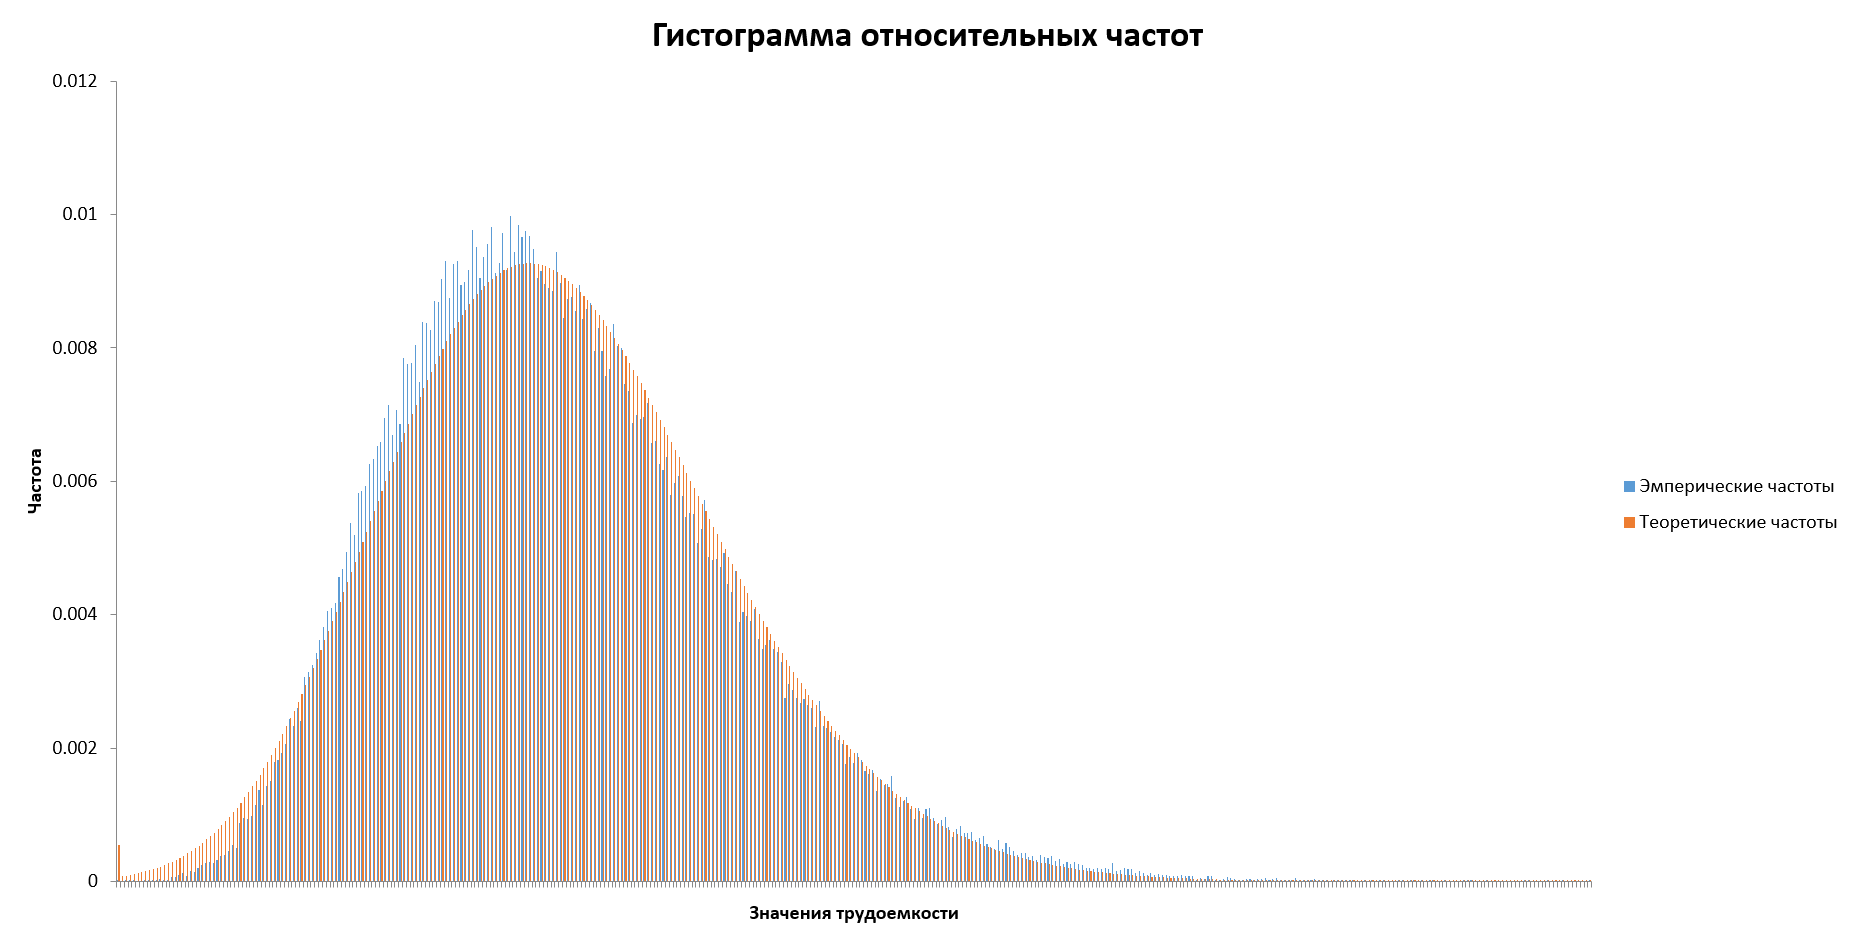
\includegraphics[width=\linewidth]{histogram.png}}
	\caption{Теоретические и эмпирические частоты для алгоритма Паллоттино при $n = 80$ с разбиением нормированного сегмента [0, 1] на 387 полусегментов}
	\label{fig:histogram}
\end{figure}

Результаты расчетов теоретических частот по функции плотности приведены на рис.~\ref{fig:histogram}. Наблюдаемое значения критерия Пирсона в данном случае $\chi_{\text{набл}}^2 = 282.24386$. Поскольку $\chi_{\text{кр}}^2(0.05, 384) = 430.69192$ (вычислено стандартной функцией пакета Microsoft Excel), получаем $\chi_{\text{набл}}^2 < \chi_{\text{кр}}^2(0.05, 384)$. Следовательно, нет оснований отвергать нулевую гипотезу и можно перейти к основному этапу исследования.

\subsection{Этап основного исследования}\label{sec:analysis_part_2}

\subsubsection{Основные этапы}\label{subsec:analysis_part_2_intro}

\begin{enumerate}
	\item Определение сегмента значений длин входа, соответствующего особенностям применения данного алгоритма в разрабатываемой
	программной системе. В данном случае алгоритма Паллоттино будет применяться для массивов длиной от 80 до 2560;

	\item Определение сегмента значений длин входа, для которого будут проводиться экспериментальные исследования. В данном примере таким сегментом является сегмент от 80 до 320;

	\item Выбор шага изменения длины входа в экспериментальном исследовании. В данном случае значение шага равно 10;

	\item Выбор необходимого числа $m$ экспериментов с программной реализацией алгоритма для фиксированной длины входа для определения выборочной средней и дисперсии. В данном случае по результатам предварительного исследования $m = 104435$;

	\item Расчет на основе экспериментальных данных значений выборочной средней и дисперсии для каждого значения $n$. В данном случае $n$ изменяется от 80 до 320 с шагом 10;

	\item Анализ экспериментальных данных~--- построение уравнения регрессии для выборочной средней и выборочной дисперсии;

	\item Расчет на основе полученных результатов параметров аппроксимирующего бета"=распределения по формулам~\eqref{eq:alpha},~\eqref{eq:beta} как функций длины входа $\alpha(n), \beta(n)$;
	
	\item Выбор значения доверительной вероятности и вычисление значений левого $\gamma$"=квантиля бета"=распределения~\cite{petrushyn_ulyanov_definitions}: $x_\gamma(n) = B^{-1}(\gamma, \alpha(n), \beta(n))$;

	\item Вычисление значений функции доверительной трудоемкости для исследуемого сегмента длин входа по формуле~\cite{petrushyn_ulyanov_analysis}:

	\begin{equation}\label{eq:final_complexity_fucntion}
		f_\gamma(n) = f^\vee(n) + x_\gamma(n) (f^\wedge(n) - f^\vee(n)).
	\end{equation}
\end{enumerate}

\subsubsection{Результаты основного исследования}\label{subsec:results_part_2}

Было проведено основное исследование с выборками объемом 104435 для входных данных в сегменте $n = [80, 2560]$. Результаты представлены на рисунках~\ref{fig:regression_mean}--\ref{fig:comparison_complexities}.

Результаты построения уравнения регрессии для нормированной выборочной средней и выборочной дисперсии показаны на рис.~\ref{fig:regression_mean} и рис.~\ref{fig:regression_varience} соответственно. В первом случае уравнение регрессии имеет вид $\overline{t} = 0.9449 \cdot n^{-1.1735}$, во втором~--- $s^2 = y = 0.1165 \cdot n^{-3.741}$. В данном случае $y = ax^{-b}$~--- наилучший в смысле максимума значения коэффициента детерминации $R^2$ вид функции, подбор коэффициентов осуществлен с помощью метода наименьших квадратов (расчеты выполнены в Microsoft Excel).

\begin{figure}[h]
	\center{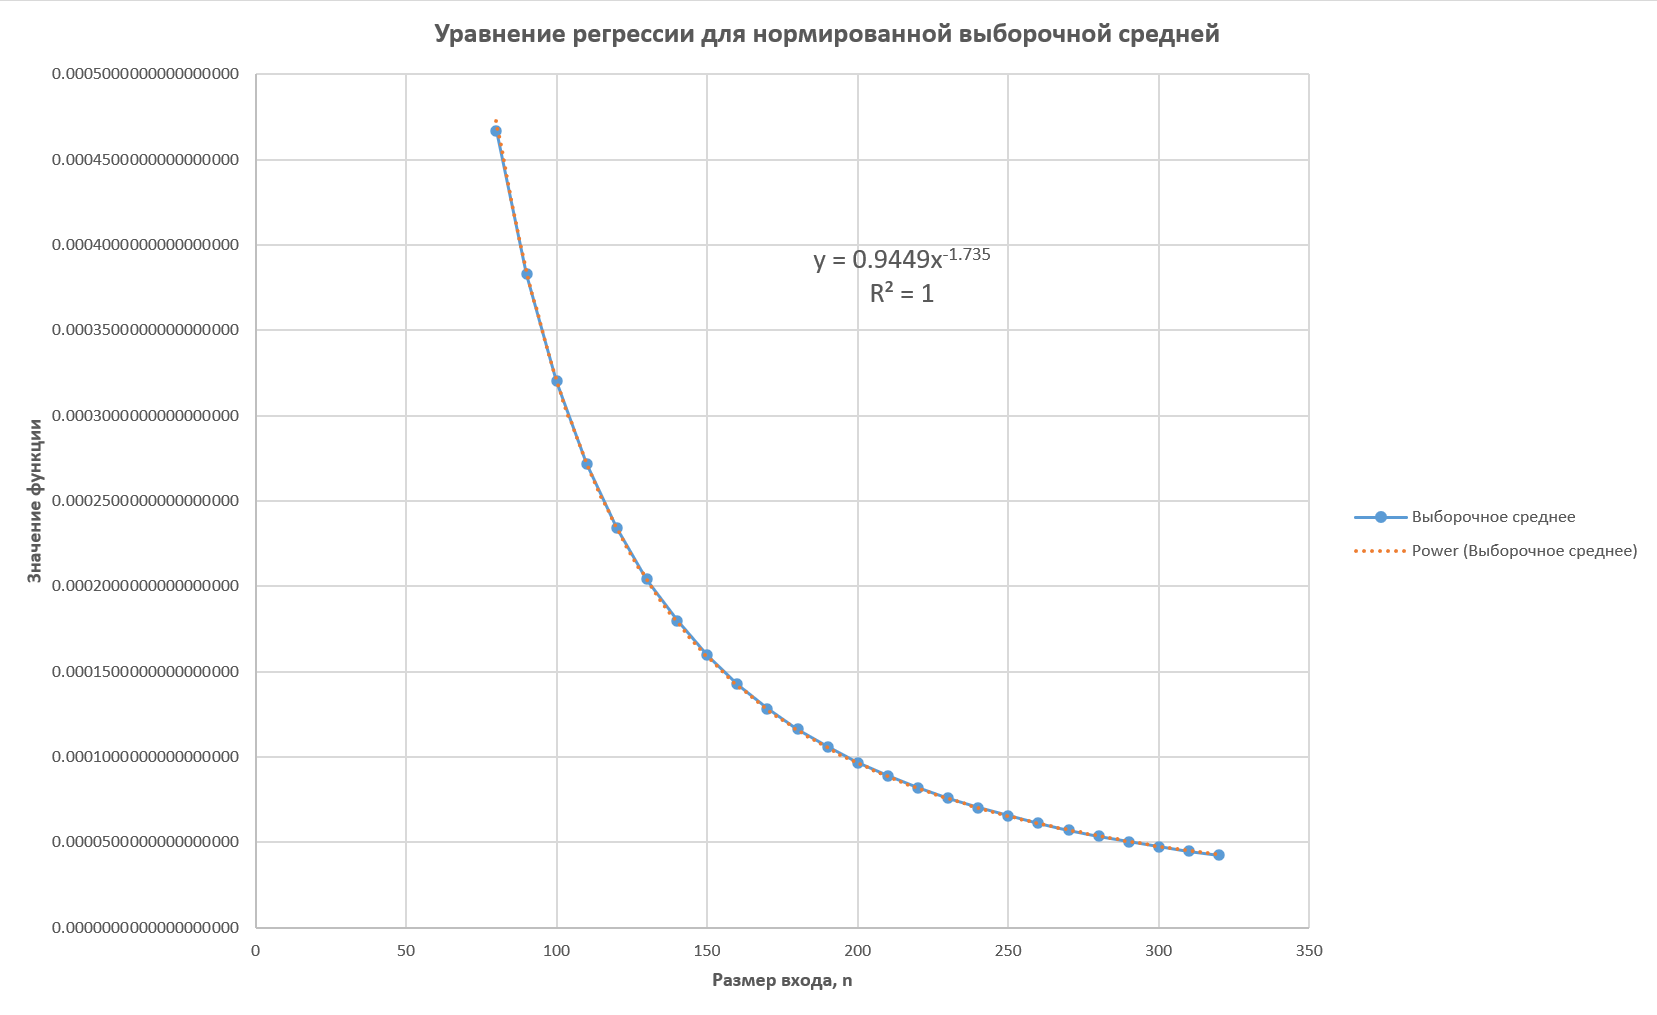
\includegraphics[width=\linewidth]{prediction_mean.png}}
	\caption{Экспериментальные данные и уравнение регрессии для нормированной выборочной средней значений трудоемкости алгоритма Паллоттино}
	\label{fig:regression_mean}
\end{figure}

\begin{figure}[h]
	\center{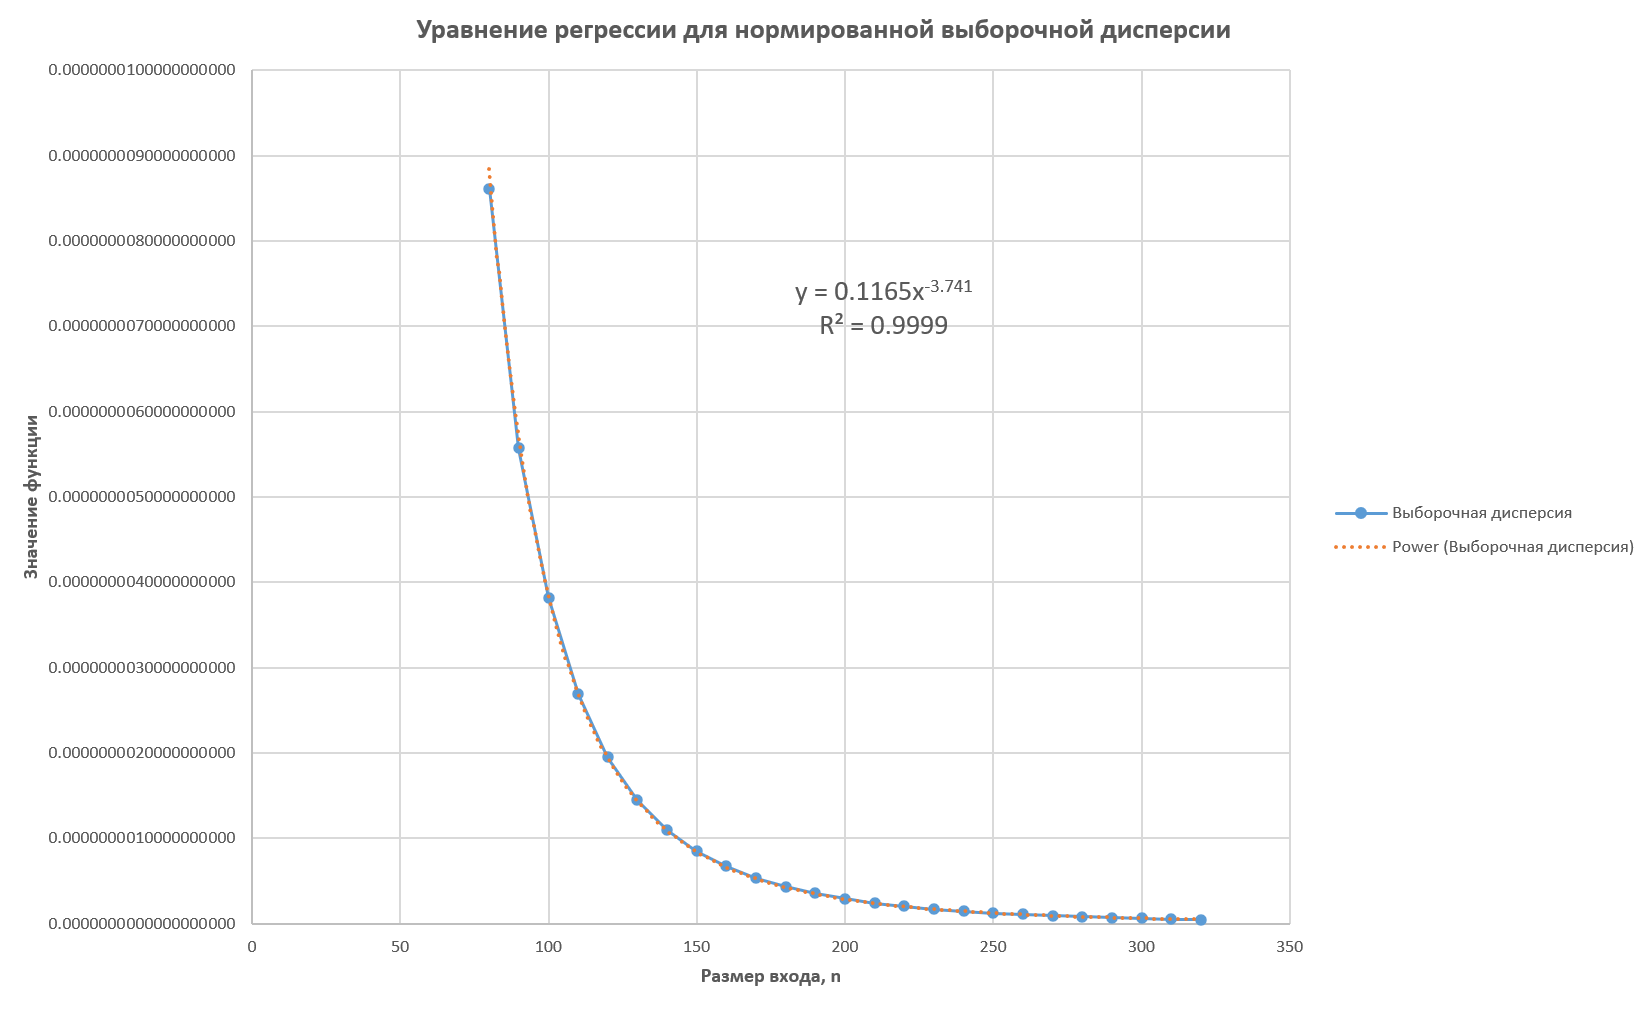
\includegraphics[width=\linewidth]{prediction_variance.png}}
	\caption{Экспериментальные данные и уравнение регрессии для нормированной выборочной дисперсии значений трудоемкости алгоритма Паллоттино}
	\label{fig:regression_varience}
\end{figure}

График функции $\alpha(n)$ показан на рис.~\ref{fig:alpha_plot}, график функции $\beta(n)$ показан на рис.~\ref{fig:beta_plot}.

\begin{figure}[h]
	\center{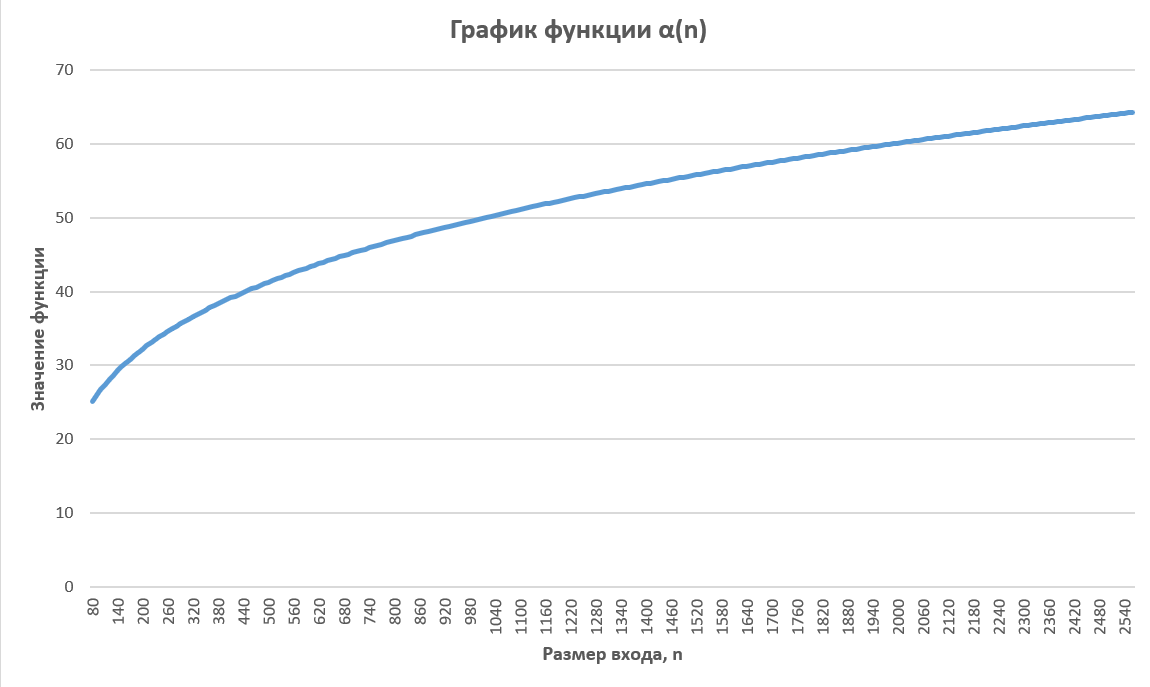
\includegraphics[width=\linewidth]{alpha.png}}
	\caption{График функции $\alpha(n)$~--- параметра $\alpha$ аппроксимирующего бета"=распределения для алгоритма Паллоттино}
	\label{fig:alpha_plot}
\end{figure}

\begin{figure}[h]
	\center{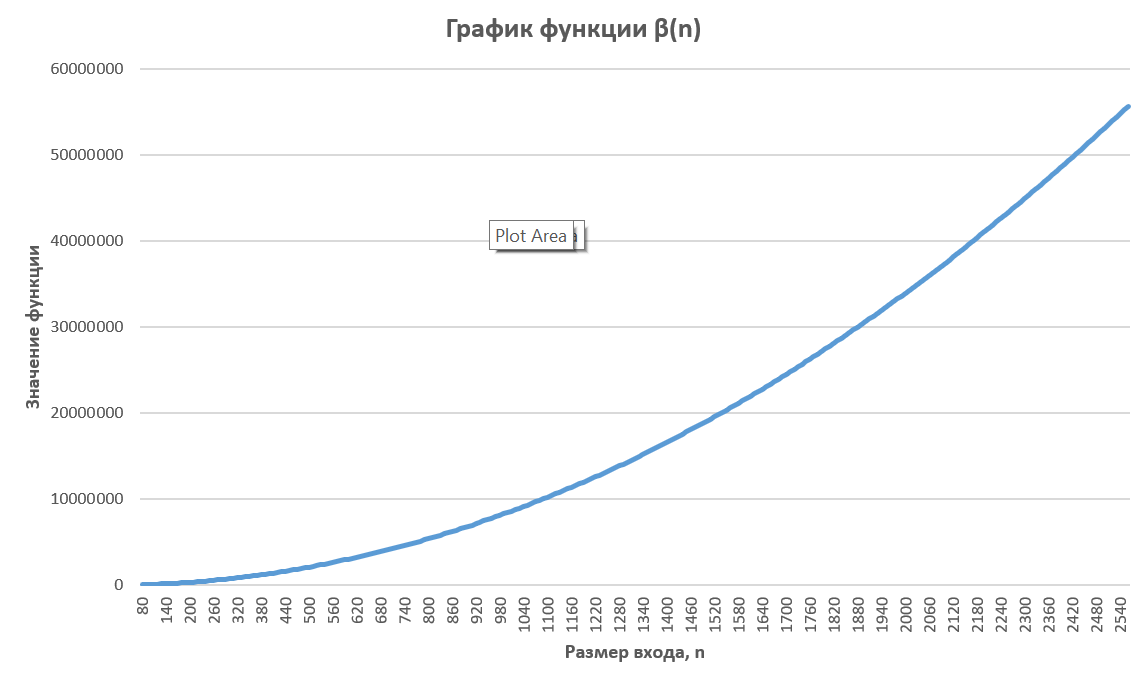
\includegraphics[width=\linewidth]{beta.png}}
	\caption{График функции $\beta(n)$~--- параметра $\beta$ аппроксимирующего бета"=распределения для алгоритма Паллоттино}
	\label{fig:beta_plot}
\end{figure}

В рассматриваемом примере $\gamma = 0.95, \alpha < \beta$, график значений $x_\gamma(n)$ показан на рис.~\ref{fig:left_quantile}. На рис.~\ref{fig:comparison_complexities} показан график значений доверительной трудоемкости и трудоемкости в худшем случае для алгоритма Паллоттино на сегменте $n = [80, 2560]$. Отдельно отметим, что доверительная трудоемкость получена для значения доверительной вероятности $\gamma = 0.95$, т.~е. в 95\% случаев наблюдаемая в единичном эксперименте трудоемкость алгоритма не будет превышать значение доверительной трудоемкости. Для рассматриваемого примера эти значения в разы меньше трудоемкости в худшем случае на исследуемом сегменте длин входа.

\begin{figure}[h]
	\center{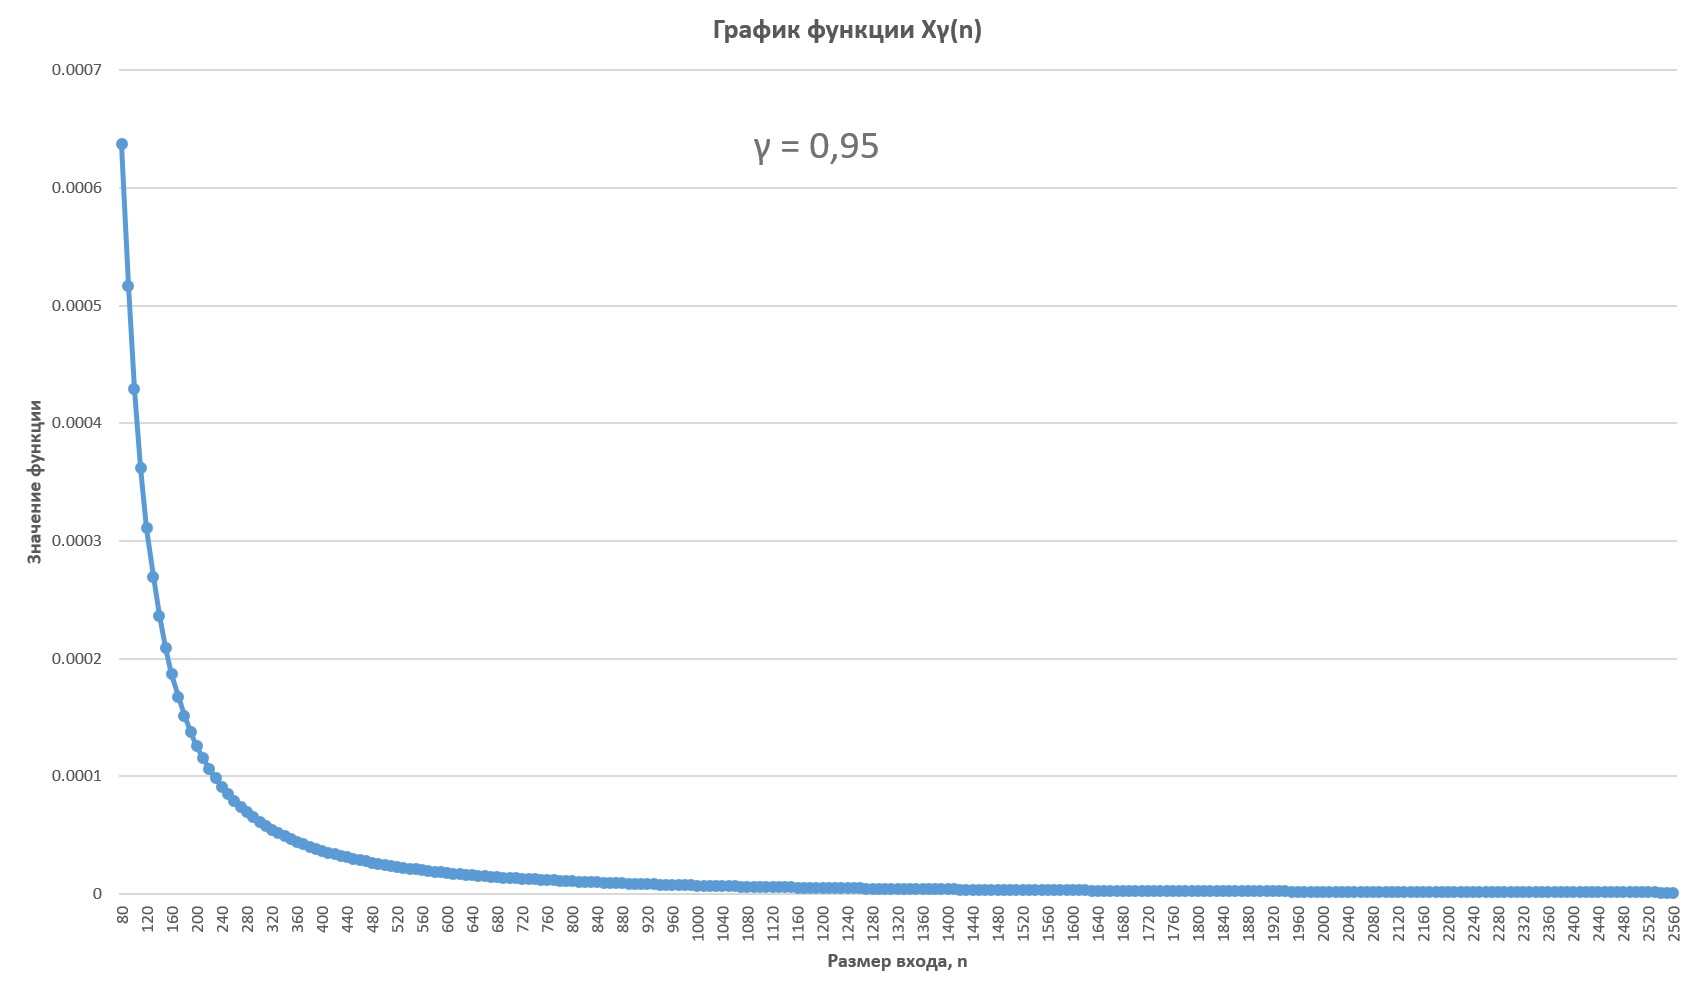
\includegraphics[width=\linewidth]{quantile.png}}
	\caption{График зависимости левого $\gamma$"=квантиля бета"=распределения $x_\gamma(n)$ от длины входа для алгоритма Паллоттино}
	\label{fig:left_quantile}
\end{figure}

\begin{figure}[h]
	\center{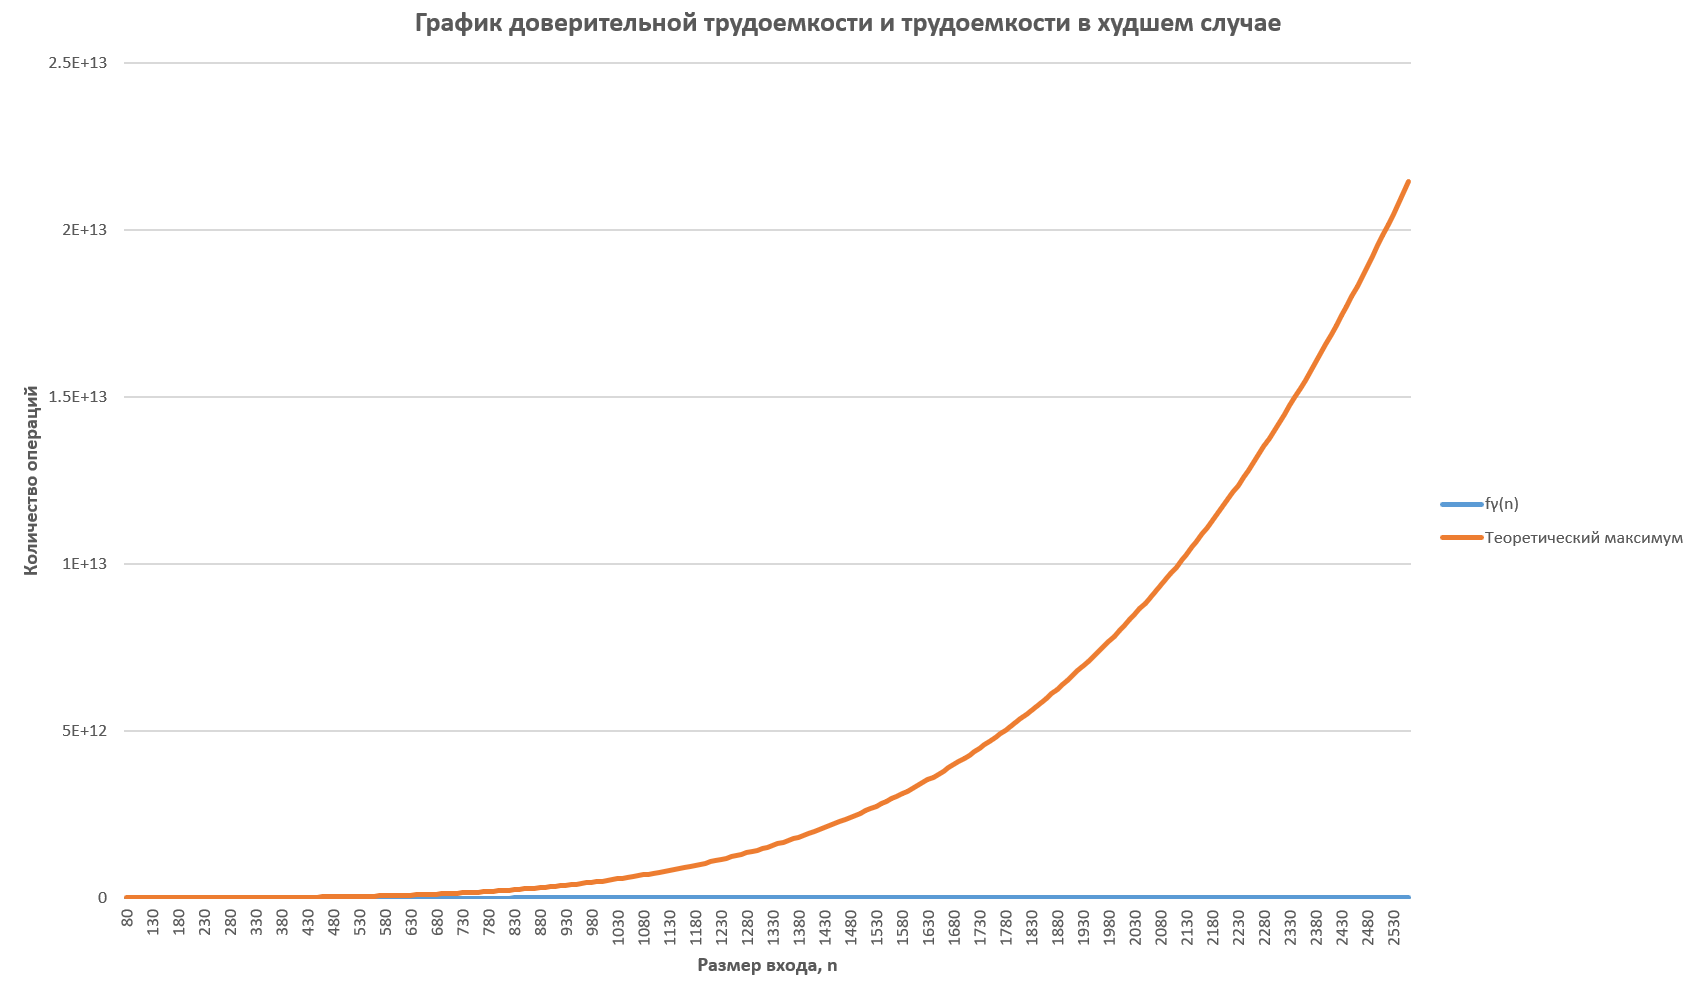
\includegraphics[width=\linewidth]{comparison.png}}
	\caption{График доверительной трудоемкости и трудоемкости в худшем случае для алгоритма Паллоттино}
	\label{fig:comparison_complexities}
\end{figure}

\section{Создание инструментария}\label{sec:analysis_system}

Реализация инструментария включает разработку desktop"=приложения на языке программирования C\# с функцией формирования отчетов в виде документа для программного пакета Microsoft Excel.

\subsection{Постановка задачи}\label{sec:technical_task}

В соответствии с описанным ранее критерием оценки по доверительной трудоемкости необходимо создать автоматизированную систему для проведения следующих этапов исследования программной реализации алгоритмов:

\begin{enumerate}
	\item[•] предварительный этап, целью которого является проверка гипотезы о виде закона распределения значений трудоемкости алгоритма как дискретной ограниченной случайной величины~\cite{petrushyn_ulyanov_planning};

	\item[•] основной этап, в ходе которого значения доверительной трудоемкости вычисляются в зависимости от длины входных данных алгоритма~\cite{petrushyn_ulyanov_analysis};

	\item[•] этап обработки результатов анализа;

	\item[•] оформление результатов анализа алгоритма в виде отчета, включающего итоговые значения требуемых вычислительных ресурсов для входных данных определенной размерности.
\end{enumerate}

Необходимо отметить, что предполагается наличие реализации компьютерного алгоритма, которая используется для проведения анализа. Также модуль с реализацией должен содержать компонент для генерации входных данных.

\subsection{Архитектура системы}\label{sec:arhitecture}

Одной из главных задач является проектирование системы с учетом поддержки наибольшего количества программных реализаций алгоритмов для проведения анализа.

Для выполнения этого требования программный модуль должен иметь определенный интерфейс, т.\,е. принимать аргументы из командной строки. Они требуются для проведения экспериментальных исследований трудоемкости в различных конфигурациях алгоритма. При этом функциональность, связанная с генерацией допустимых входных данных также должна находиться в программном модуле. Система передает только параметры, содержащие размер требуемой выборки и границы сегментов для проведения экспериментов.

В процессе разработки использованы следующие технологии: Windows Presentation Foundation (WPF) для реализации пользовательского интерфейса, EPPlus для формирования отчета в виде документа пакета Microsoft Excel~\cite{excel}. Такой стек технологий позволяет вести разработку и поддержку специалисту, владеющему только одним языком программирования. Схема архитектуры прототипа представлена на рис.~\ref{fig:arhitecture}.

\begin{figure}[h]
	\center{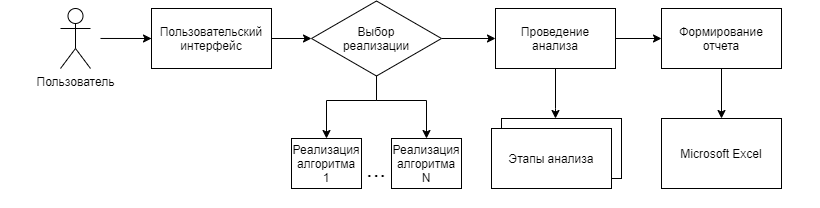
\includegraphics[width=0.98\linewidth]{arhitecture.png}}
	\caption{Схема архитектуры системы}
	\label{fig:arhitecture}
\end{figure}
\vskip4mm

\subsection{Описание реализации}\label{sec:implementation}

На основе приведенной архитектуры разработано приложение на языке C\#~\cite{system_source}, позволяющее проводить анализ алгоритмов и получать результаты в виде отчета для изучения их применимости на заданных входных данных.

В первую очередь, нужно получить программную реализацию алгоритма. Язык программирования или технологии, используемые для получения реализации, не имеют значения. Единственное требование~--- возможность принимать входные параметры для проведения экспериментальных исследований. В случае отсутствия возможности принимать параметры система не сможет провести анализ для предоставленной программной реализации.

Система имеет предопределенный набор программных реализаций алгоритмов, которые можно использовать для анализа. Для добавления новой реализации достаточно поместить разработанный модуль в каталог с установленной системой. При запуске система автоматически обнаружит новый модуль и добавит его в качестве одного из вариантов для проведения анализа.

\begin{figure}[h]
	\center{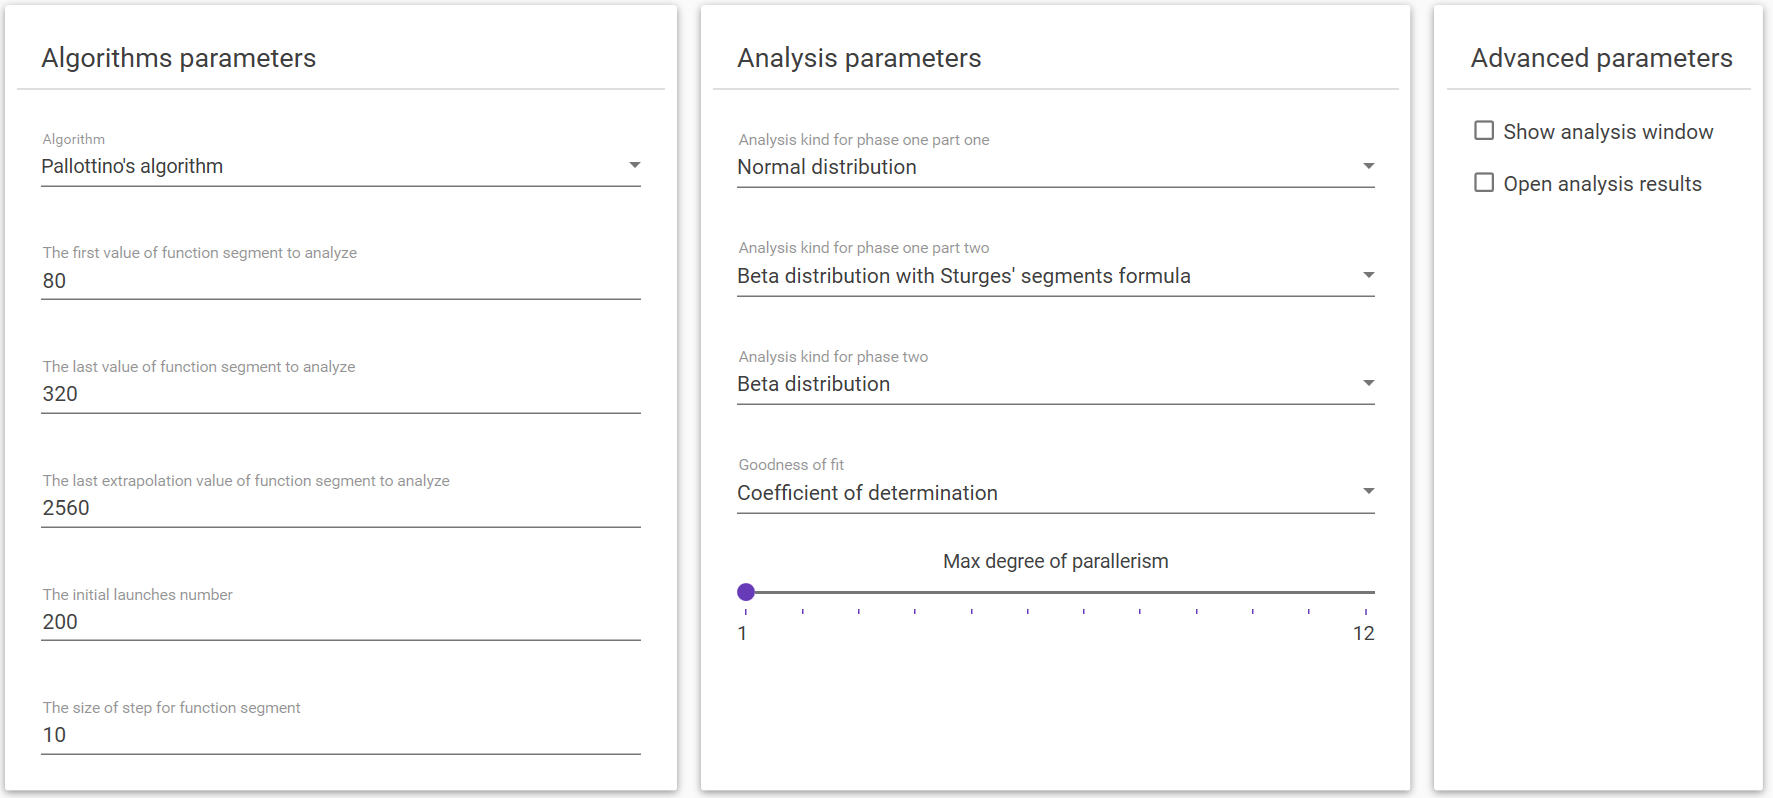
\includegraphics[width=0.9\linewidth]{interface.png}}
	\caption{Интерфейс настройки параметров анализа}
	\label{fig:interface}
\end{figure}
\vskip6mm

Предусмотрена возможность настройки системы и выбора желаемых методов расчета количества полусегментов гистограммы относительных частот, размера выборки и т.\,д. Практически все описанные в работе методы присутствуют в системе и доступны для использования. Это позволяет исследователям проверять различные гипотезы при анализе функции трудоемкости для программных реализаций алгоритмов.

\begin{figure}[h]
	\center{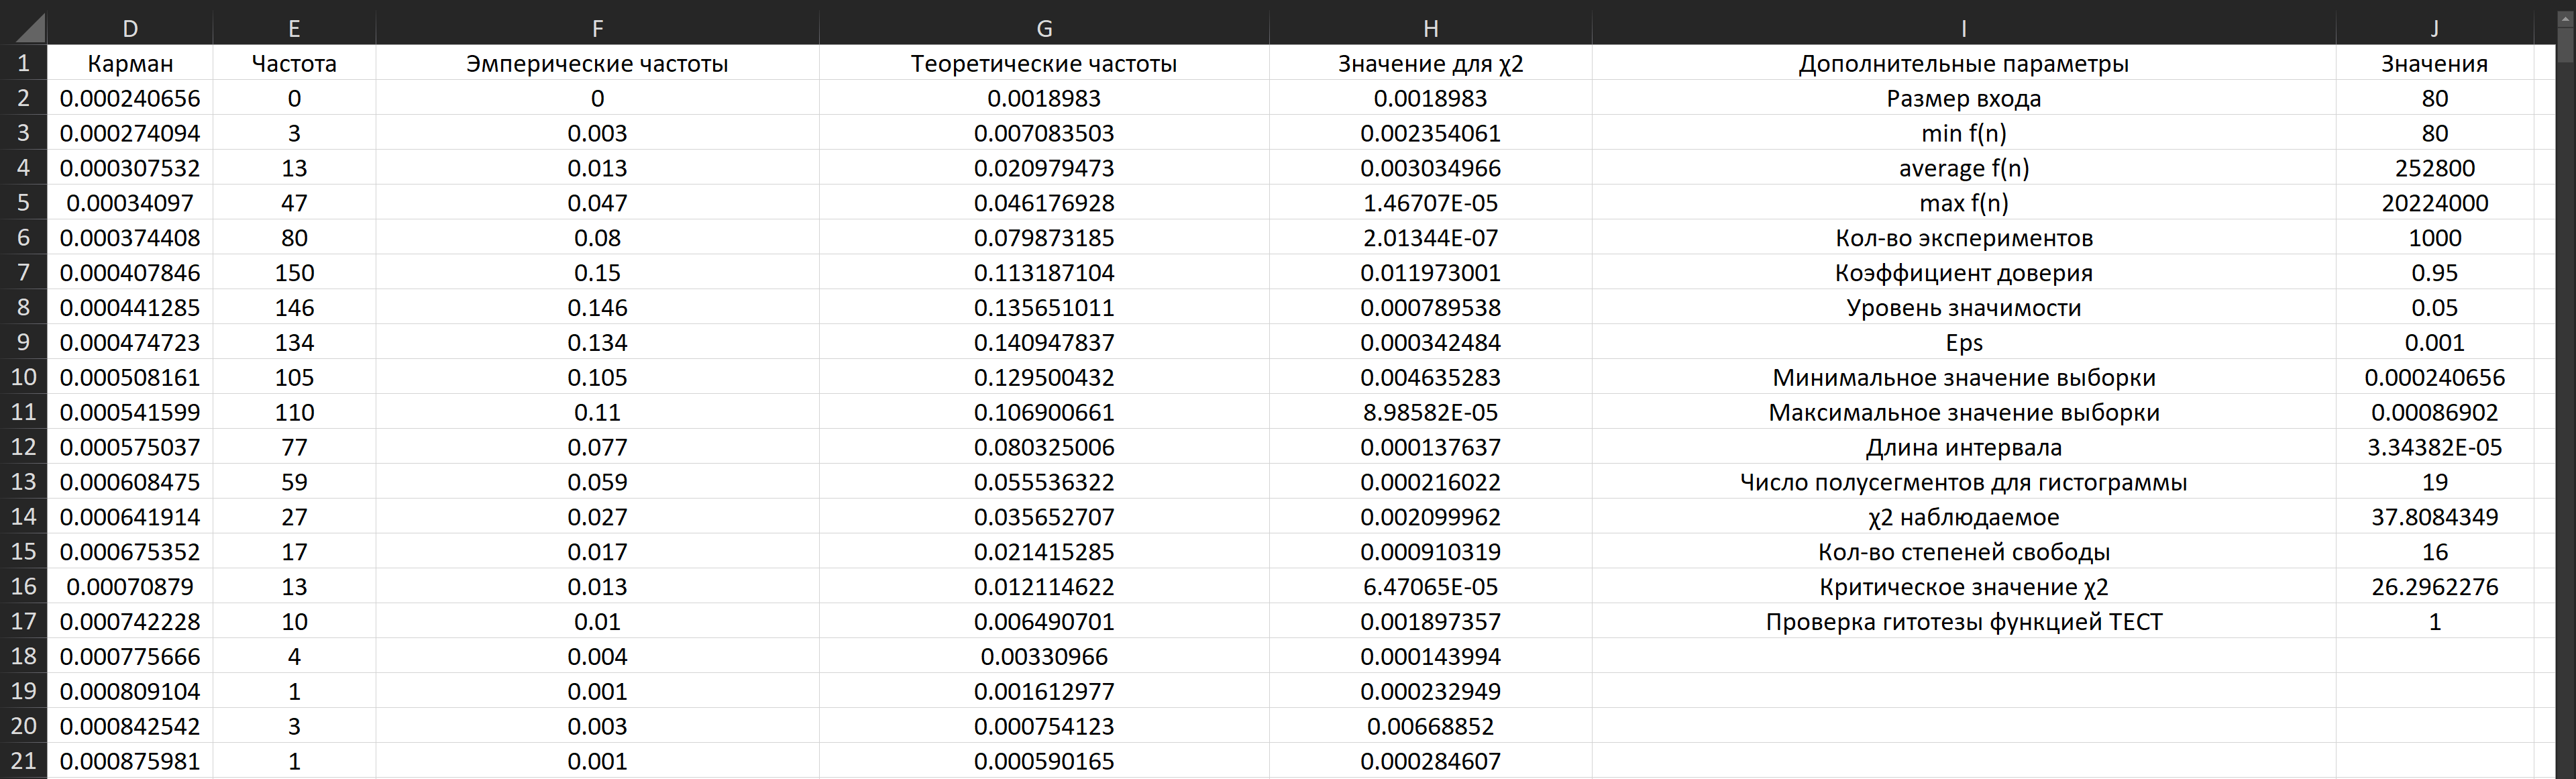
\includegraphics[width=0.95\linewidth]{results.png}}
	\caption{Пример результатов анализа}
	\label{fig:results}
\end{figure}
\vskip5mm

Параметры для экспериментальных исследований формирует система на основе пользовательского ввода и передает их программе в качестве аргументов командной строки при запуске. Пример набора параметров показан на рис.~\ref{fig:interface}. Результаты многократного запуска исследуемой программной реализации сохраняются во временный файл, из которого потом загружаются в систему для проведения основного этапа исследования. По окончании анализа формируется отчет с подробным описанием полученных оценок эффективности (рис.~\ref{fig:results}).

\specialsection{Выводы}\label{sec:conclusion}

Поставленные задачи выполнены, созданный инструментарий позволяет проводить все этапы анализа функции трудоемкости и вычислять доверительную трудоемкость.

Поставленный эксперимент с алгоритмом Паллоттино показал, что оценка функции сложности в худшем случае может приводить к существенному завышению временного прогноза из"=за малой вероятности входных данных, обеспечивающих максимум функции трудоемкости для рассматриваемой задачи. Полученные результаты подтверждают возможность повышения достоверности прогнозирования временной эффективности компьютерных алгоритмов и более эффективного решения задачи выбора рациональных алгоритмов на основе сравнительного анализа функций доверительной трудоемкости вместо традиционного сравнения трудоемкости в среднем случае.

Созданная автоматизированная система принимает на вход любые программные реализации алгоритмов, удовлетворяющих требуемому программному интерфейсу вне зависимости от выбранного языка программирования или используемых технологий разработки.

Отдельный интерес для дальнейшего исследования представляет рассмотрение алгоритмов класса NPR с функцией трудоемкости, зависящей от двух и более параметров входа. В данной работе в качестве объекта исследований был взят алгоритм Паллоттино с функцией трудоемкости от двух параметров входа (количество вершин и количество ребер). Чтобы использовать методологию, изложенную в~\cite{petrushyn_ulyanov_analysis}, потребовалось зафиксировать второй параметр. Именно поэтому в качестве входных данных рассмотрены только полные графы, для которых можно легко рассчитать количество ребер при заданном количестве вершин. Однако не всегда можно выразить один параметр функции трудоемкости через другой. Таким образом, одним из потенциальных улучшений работы является исследование функции трудоемкости при вариации нескольких параметров, что позволит применять описанную методологию к более широкому классу алгоритмов.

\specialsection{Заключение}\label{sec:summary}

Исследованы различные дополнительные методы для применения методологии~\cite{petrushyn_ulyanov_analysis} на более широкий класс алгоритмов.

Разработана автоматизированная система для оценки качества алгоритмов по доверительной трудоемкости, вычисленной в процессе эмпирического анализа программной реализации. Преимущество системы состоит в получении гарантирующей оценки на основе статистических заключений с заданным уровнем значимости. Исходный код и документация системы находятся в публичном репозитории в GitHub~\cite{system_source}.

\newpage

% Библиография в CPS Conf стиле.
% Аргумент {1} ниже включает переопределенный стиль с выравниванием слева.
%\section{Список литературы}\label{sec:sources}
\begin{thebibliography}{1}\label{sec:sources}
	% №1
	\bibitem{petrushyn_ulyanov_analysis} Петрушин~В.\:Н., Ульянов~М.\:В., Кривенцов~А.\:С. Доверительная трудоемкость~--- новая оценка качества алгоритмов // Информационные технологии и вычислительные системы. 2009. \No~2. С.~23--37.

	% №2
	\bibitem{trachtenbort_common} Трахтенброт Б. А. Сложность алгоритмов и вычислений. Новосибирск: Изд"=во Новосибирского ун"=та, 1967.

	% №3
	\bibitem{ofman} Офман~Ю.\:П. Об алгоритмической сложности дискретных функций // ДАН СССР. 1962. Т.~45, вып.~1. С.~48--51.

	% №4
	\bibitem{caytin} Цейтин~Г.\:С. Оценка числа шагов при применении нормального алгоритма // Математика в СССР за 40 лет. Т.~1. М., 1959. С.~44--45.

	% №5
	\bibitem{trachtenbort_recursion} Трахтенброт~Б.\:А. Сигнализирующие функции и табличные операторы // Записки Пензенского ГПИ. 1956. Вып.~4. С.~75--87.
	
	% №6
	\bibitem{alpherova} Алферова~З.\:В. Теория алгоритмов. М.: Статистика, 1973.

	% №7
	\bibitem{gashkov} Гашков~С.\:Б., Чубариков~В.\:Н. Арифметика. Алгоритмы. Сложность вычислений: Учеб. пособие для вузов / Под ред. В.~А.\:Садовничего. 2"=е изд., перераб. М.: Высш. шк., 2000.

	% №8
	\bibitem{cormen} Cormen~T.\:H., Leiserson~C.\:E., Rivest~R.\:L., Stein~C. Introduction to Algorithms. Chapter 1: Foundations (Second ed.) // Cambridge, MA: MIT Press and McGraw-Hill. 2001. P.~3--122.

	% №9
	\bibitem{knuth} Knuth~D. The Art of Computer Programming / Addison\,--\,Wesley, 1968.

	% №10
	\bibitem{wegener} Wegener~I. Complexity theory: exploring the limits of efficient algorithms // Berlin, New York: Springer\,--\,Verlag. P.~20.

	% №11
	\bibitem{juraj} Juraj~H. Theoretical computer science: introduction to Automata, computability, complexity, algorithmics, randomization, communication, and cryptography // Springer. 2004. P.~177--178.

	% №12
	\bibitem{berube} Berube~P., Amaral~J.\:N. Combined profiling: A methodology to capture varied program behavior across multiple inputs // ISPASS 2012~--- IEEE International Symposium on Performance Analysis of Systems and Software. 2012. No~6189227. P.~210--220.

	% №13
	\bibitem{runtime_prediction} Hutter~F., Xu~L. Hoos~H., Leyton\,--\,Brown~K. Algorithm runtime prediction: Methods \& evaluation // Artificial Intelligence. 2014. Vol.~206. No~1. P.~79--111.

	% №14
	\bibitem{intelligence_forecasting} Oprea~M. A general framework and guidelines for benchmarking computational intelligence algorithms applied to forecasting problems derived from an application domain-oriented survey // Applied Soft Computing. 2020. Vol.~89. No~4. P. 106--103.

	% №15
	\bibitem{petrushyn_ulyanov_planning} Петрушин~В.\:Н., Ульянов~М.\:В. Планирование экспериментального исследования трудоемкости алгоритмов на основе бета"=распределения // Информационные технологии и вычислительные системы. 2008. \No~2. С.~81--91.

	% №16
	\bibitem{functional_nuprl} Benzinger~R. Automated complexity analysis of Nuprl extracted programs // Journal of Functional Programming. 2001. Vol.~11. No~1. P.~3--31.
	
	% №17
	\bibitem{functional_automation} Hickey~T., Cohen~J. Automating program analysis // Journal of the ACM. 1988. Vol.~35. No~1. P.~185--220.

	% №18
	\bibitem{petrushyn_ulyanov_definitions} Петрушин~В.\:Н., Ульянов~М.\:В. Информационная чувствительность компьютерных алгоритмов. М.: Физматлит, 2010.

	% №19
	\bibitem{gmurman} Гмурман~В.\:Е. Теория вероятностей и математическая статистика: Учеб. пособие для вузов, 9"=е изд., стер. М.: Высш. шк., 2003.

	% №22
	\bibitem{scott} Scott~D.\:W. On optimal and data-based histograms // Biometrika. 1979. Vol.~66. P.~605--610.
	
	% №23
	\bibitem{freedman_diaconis} Freedman~D., Diaconis~P. On the histogram as a density estimator: 12 theory // Z. Wahrscheinlichkeit. 1981. Vol.~57. P.~453--476.

	% №20
	\bibitem{sturges} Sturges~H. The choice of a class-interval // J. Amer. Statist. Assoc. 1926.
	Vol.~21. P.~65--66.

	% №21
	\bibitem{hyndman} Hyndman~R.\:J. The problem with Sturges' rule for constructing histograms // The Pennsylvania State University. 1995.

	% №24
	\bibitem{koroluk} Королюк~В.\:С., Портенко~Н.\:И., Скороход~А.\:В., Турбин~А.\:Ф. Справочник по теории вероятностей и математической статистике. М.: Наука, 1985.

	% №25
	\bibitem{prohorov} Прохоров~Ю.\:В., Розанов~Ю.\:А. Теория вероятностей (Основные понятия. Предельные теоремы. Случайные процессы). М.: Наука. Физматлит, 1987.

	% №26
	\bibitem{arsenin} Арсенин~В.\:Я. Математическая физика: основные уравнения и специальные функции. М.: Наука, 1966.

	% №27
	\bibitem{smirnov} Смирнов~Н.\:В., Дунин\,--\,Барковский~И.\:В. Краткий курс математической статистики для технических приложений. М.: Физматгиз, 1959.

	% №28
	\bibitem{kac} Kac~M., Kiefer~J., Wolfowitz~J. On Tests of Normality and Other Tests of Goodness of Fit Based on Distance Methods // Ann. Math. Stat., 1955. Vol.~26. P.~189--211.

	% №29
	\bibitem{hughes} Hughes~A., Grawoig~D. Statistics: A Foundation for Analysis / Addison\,--\,Wesley, 1971.

	% №30
	\bibitem{dijkstra} Dijkstra~E.\:W. A note on two problems in connexion with graphs // Numer. Math. 1959. Vol.~1. P.~269--271.

	% №31
	\bibitem{bellman} Bellman~R. On a routing problem // Quart. Appl. Math. 1958. Vol.~16. P.~87--90.

	% №32
	\bibitem{ford} Ford~L.\:R. and Fulkerson~D.\:R. Flows in Networks // Princeton:~Princeton University Press. 1962.

	% №33
	\bibitem{moore} Moore~E.\:F. The shortest path through a maze // Bell Telephone System. Technical publications. 1959. Vol.~3523.

	% №34
	\bibitem{desopo} Pollack~M. and Wiebenson~W. Solutions of the shortest"=route problem – A review // Oper. Res. 8. 1960. P.~224--230.

	% №35
	\bibitem{pape} Pape~U. Implementation and efficiency of Moore"=algorithms for the shortest route problem // Math. Program. 1974. Vol.~7. P.~212--222.

	% №36
	\bibitem{levit_livshits} Левит~Б.\:Ю., Лившиц~В.\:Н. Нелинейные сетевые транспортные задачи // Институт комплексных транспортных проблем. М., Изд"=во «Транспорт». 1972. С.~1--144.

	% №37
	\bibitem{pallottino} Pallottino~S. Shortest"=path methods: Complexity, interrelations and new propositions // Networks. 1984. Vol.~14. P.~257--267.
	
	% №38
	\bibitem{excel} Приложение для работы с электронными таблицами Microsoft Excel [Электронный ресурс]: \url{URL: https://products.office.com/ru-ru/excel} (дата обращения: 30.04.2020).

	% №39
	\bibitem{system_source} Репозиторий проекта в системе контроля версий GitHub [Электронный ресурс]: \url{URL: https://github.com/Vasar007/algorithm_analysis} (дата обращения: 30.04.2020).

\end{thebibliography}

\end{document}
